\documentclass[german,version-2022-01]{uzl-thesis}


% Copy this file as a template for your thesis. You will have to take
% action at all places marked by
%
% !!!!!!!!!!!!!!!!!!!!!!!!!!!!!!!!!!
% !!! Your action is needed here !!!
% !!!!!!!!!!!!!!!!!!!!!!!!!!!!!!!!!!
%
% The first place your action is needed is the first line of this
% document:
%
%
% Language of the thesis:
%
% You must use either 'german' or 'english' above, depending on the
% language used in the main text. This will automatically setup a lot 
% of things in the background.
%
%
% Version of the class:
%
% You must specify which version of the thesis class is to be
% used. This is important in case the class style changes in later
% years, but we still want an older thesis to look the same, even when
% things are changed in the class.
%
% Do not change or remove the version-xxxx key.
%
%
% Text encoding:
%
% Your thesis *must* be encoded in utf8 (unicode), which is the
% default in most editors these days. Do *not* change this to latin8.



%%%
%
% Main setup:
%
%%%
%
% You must use the \UzLThesisSetup command to specify numerous things
% about your thesis. This includes the entries on the title page, the 
% abstracts, and the bibliography style. You do so by specifying
% so-called "values" for so-called "keys". For instance, 
% for the key "Autor" you must provide your name as the value. You do
% so by writing 'Autor = {Max Mustermann}', that is, the value is put
% into curly braces. You can use the \UzLThesisSetup command
% repeatedly and the order in which you provide the keys is not
% important. 
%
% Everything shown on the title page must be in German -- even
% if the thesis is written in English! Just insert German text for
% German keys and English text for English keys (like 'Abstract' needs
% English text, while 'Zusammenfassung' needs German text).

\UzLThesisSetup{
  %
  % !!!!!!!!!!!!!!!!!!!!!!!!!!!!!!!!!!
  % !!! Your action is needed here !!!
  % !!!!!!!!!!!!!!!!!!!!!!!!!!!!!!!!!!
  %
  % First, specify the institut or clinic at which the thesis was
  % written. You get the logo file from them (make sure it has the
  % correct size, namely the same as the example). If they do not have
  % a logo, the university's default logo is used.
  %
  % The 'verfasst' gets two arguments. Change the first to {an der}
  % for clinics, as in 'Verfasst = {an der}{Medizinischen Klinik I}'
  %
  Logo-Dateiname        = {Logo_INB_600dpi.png},
  Verfasst              = {am}{Institut f\"ur Neuro- und Bioinformatik},
  %
  % The titles:
  %
  Titel auf Deutsch     = {
    Analyse einer DNA-Datenbank auf Mutationsstabilit\"at basierend auf (bio-)chemisch relevanter Molek\"uleigenschaften
  }, 
  Titel auf Englisch    = {
    Analysis of a DNA Database for Mutation Stability Based on (Bio-)Chemically Relevant Molecular Properties 
  },
  %
  % Author and supervisor:
  % 
  % Note that the 'Betreuer' or 'Betreuerin' is the supervisor, that
  % is, the professor who officially supervises the thesis. If there
  % is also an assistent of the professor who helped (typically a
  % lot), use 'Mit Unterstützung von' to thank that person. If the
  % thesis was mainly written 'externally' at some company or another
  % institute, point this out using 'Weitere Unterstützung'. 
  % 
  % For your own name, do *not* add things like "BSc" or "BSc
  % cand.". For the supervisor, you should normally include
  % "Prof. Dr." or "PD Dr." (ask your supervisor, what is
  % appropriate), but nothing more (so no
  % "Univ.-Prof. Dr. Dr. h.c. mult." unless your supervisor insists).  
  %
  Autor                 = {Leonie Nie\ss{}},
  Betreuerin            = {PD Dr. Amir Madany Mamlouk},
  % 
  % Optional: Supporting persons and institutions. The text should be
  % in German, even for an English thesis.
  %
  Mit Unterstützung von = {B.Sc. Nina Eichler},
  % 
  %   Weitere Unterstützung = {
  %     Die Arbeit ist im Rahmen einer Tätigkeit bei der Firma Muster GmbH
  %     entstanden.
  %   },
  %
  %
  % Your Degree Programm (Studiengang)
  %
  % Specify 'Bachelorarbeit' or 'Masterarbeit' and the degree
  % programme. Make sure the name of programme is correct and not
  % some abbreviation or some incorrect variant. For instance:
  % 'Medizinische Ingenierwissenschaft', but not 'MIW';
  % 'Medizinische Informatik', but not 'Medizin-Informatik';
  % 'Informatik', but not 'Informatik (SSE)'.
  %
  % Use German names for German programmes and English names for
  % English ones, so 'Infection Biology', not 'Infektionsbiologie'. 
  % For programmes that have a German bachelor and an English master,
  % use the German name for a bachelor thesis and the English name for
  % the master thesis.
  %
  Bachelorarbeit,
  Studiengang           = {Medizinische Informatik},
  %
  % Date on which the thesis is turned in German, formatted the
  % traditional German way:
  %
  Datum                 = \today,
  %
  % The English abstract. You must always provide abstracts in German
  % and in English. 
  %
  Abstract              = {
    Hydrophobic and hydrophilic properties are essential for the interaction of transmembrane proteins with their environment and can be quantified through hydropathy and polar-requirements values. In this bachelor's thesis, the stability of transmembrane regions within viral proteins, specifically the dengue virus, is investigated in relation to hydropathy and polar-requirements values. By examining differences in polar-requirements and hydropathy values across the four dengue serotypes, ten specific proteins were assessed for mutation stability, revealing significant conservation in the transmembrane proteins NS3 and NS4B, indicating evolutionary pressure. In contrast, the transmembrane protein NS2A exhibited high mutation rates and did not show similar conservation. These findings underscore the necessity for further research, such as investigating individual protein domains to better understand their mutation patterns.
  },
  Zusammenfassung       = {
    Hydrophobe und hydrophile Eigenschaften sind entscheidend f\"ur die Interaktion von Transmembranproteinen mit ihrer Umgebung und k\"onnen durch Hydropathie und Polar-Requirement-Werte quantifiziert werden. In dieser Bachelorarbeit wird die Stabilit\"at von Transmembranbereichen innerhalb von Virusproteinen, insbesondere des Dengue-Virus, in Bezug auf Hydropathie und Polar-Requirement-Werte untersucht. Durch die Untersuchung der Unterschiede in den Polar-Requirement- und Hydropathiewerten zwischen den vier Dengue-Serotypen wurden zehn spezifische Proteine auf Mutationsstabilit\"at bewertet, wobei eine signifikante Konservierung in den Transmembranproteinen NS3 und NS4B festgestellt wurde, was auf einen evolution\"aren Druck hinweist. Im Gegensatz dazu wies das Transmembranprotein NS2A hohe Mutationsraten auf und zeigte nicht dieselbe Konservierung. Diese Ergebnisse verdeutlichen die Notwendigkeit weiterer Forschung, wie beispielsweise die Untersuchung einzelner Proteindom\"anen, um deren Mutationsmuster besser zu verstehen.
  },
  %
  % Optional: 'Danksagungen' (German) or 'Acknowledgements'
  % (English). Both keys are optional and both have the same effect of
  % adding an acknowledgements text after the abstracts and before the
  % table of contents.
  %
  %Acknowledgements      = {
  %  This is the place where you can thank people and institutions, do not try to do this on the title page. The only exception is in case you wrote your thesis while working or staying at a company or abroad. Then you should use the \Latex{Weitere Unterstützung} key to provide a text (in German) that acknowledges the company or foreign institute. For instance, you could use texts like »Die Arbeit ist im Rahmen einer Tätigkeit bei der Firma Muster GmbH entstanden« or »Die Arbeit ist im Rahmen eines Forschungsaufenthalts beim Institut für Dieses und Jenes an der Universität Entenhausen entstanden«. Do not name and thank individual persons from the company or foreign institute on the title page, do that here. 
  %},
  % Bibliography style: Choose between
  % 
  % 'Alphabetische Bibliographie'
  % for all degree programmes in the natural sciences 
  % 
  % 'Numerische Bibliographie'
  % alternative for all other degree programmes
  % 
  % Either will load biblatex and setup the citation methods and the
  % bibliography styles correctly. You should not mess with them.
  % 
  % Alphabetische Bibliographie,
  % Alternatively:
  Numerische Bibliographie
}




%%%%%%%%%%%%%%%%%%%%
%
% Styling the thesis
%
%%%%%%%%%%%%%%%%%%%%
%
% Creating a visually pleasing layout and choosing fonts is not
% easy. Furthermore, different people have different preferences. Of
% course, for the University of Lübeck, the dean of studies could just
% force everyone to use one specific layout and font, but that seems a
% bit drastic and, also, it seems nice that thesis by different people
% have an individual style even though they all stick to the same
% overall structure.
%
% For these reasons, I (Till Tantau) have spend quite some time on
% designing a flexible layout and styling mechanism for theses.
%
% Basically, the overall structure of the thesis is fixed by the
% thesis class and so are many structural elements. For instance, you
% cannot change the order in which the abstract and table of contents
% are shown, you cannot move the bibliography elsewhere, indeed, the
% bibliography style is also fixed. Likewise, the text on the title
% page is fixed.
%
% Although many things are fixed, you *can* change several other
% things. For instance, you can change the font used for the main
% text, you can change which font is used for titles and headings or
% you can change whether titles and headlines are centered or flushed
% left.
%
% There are many LaTeX packages for changing such things. You are
% kindly asked *not to use them*. Rather, use (only) the options
% offered by the thesis class. All possible choices and combinations
% there have been tested by me and produce nice results; what happens
% with other packages no one knows and might no longer conform to what
% is expected by the university. As you will see, you still have a
% lot of options.
%
%
% Technical note: All styling is done via the command
%
% \UzLStyle{...}
%
% where ... is a key-value list just as for \UzLThesisSetup. The
% difference is just that everything having to do with styling as
% controlled by \UzLStyle, while the more “formal” setup keys are
% controlled by \UzLThesisSetup.
%
%%%
%
% Designs
%
%
% A \emph{design} is a whole set of font and layout options bundled
% together. They have been chosen in such a way that a visually
% pleasing “overall appearance” results.
%
%
% \UzLStyle{computer modern oldschool design}
%
% The look of this design mimics the “classical” way a paper or report
% created with \LaTeX\ looks like: The Computer Modern font is used,
% bold face fonts are used for headlines, only black and white are
% used as colors. This design reminds me of older scientific
% documents, especially from the computer science community where
% \LaTeX\ was used very early.
%
%
% \UzLStyle{computer modern basic design}
%
% A slightly less “oldschool” version of the previous design. It is
% still a classic design in the sense that it uses the Computer Modern
% font and that it still has this “good old \LaTeX” look, but some
% more modern aspects (like colors!) have been added.
%
% Note that this design uses Myriad for the title page (one of the
% “modern aspect”), which means that his font must be installed.
%
%
% \UzLStyle{computer modern scholary design}
%
% In my opinion, this is the ultimate “scholary design”: The thesis
% will look like it has been typeset by hand some 150 years ago and
% then printed by a university press. There is really nothing “modern”
% about it and the word in the name of the design is just part of the
% name of the “Computer Modern” font.
%
%
% \UzLStyle{pagella basic design}
%
% A, well, basic design that uses the Pagella font rather than the
% Computer Modern font. Especially the bold face version of this font
% looks nicer than the Computer Modern counterpart. Also, Pagella,
% while still having a “bookish” look, still feels a bit fresher than
% Computer Modern. 
%
%
% \UzLStyle{pagella centered design}
%
% A variant of the basic Pagella design that centers all
% headlines. A nice alternative to the basic version.
%
%
% \UzLStyle{pagella contrast design}
%
% This design tries to create some visual friction by contrasting the
% sans serif headline font (in bold!) with the main text. I find it a
% visually very interesting combination.
%
%
% \UzLStyle{alegrya basic design}
%
% The third variant of the basic design, this time using the Alegrya
% font. 
%
%
% \UzLStyle{alegrya scholary design}
%
% The Alegrya version of the previous “scholary” design. Unlike the
% Computer Modern version, this design does not look old, but more
% fresh -- while still creating the impression that the text must be
% about a very scientific subject. 
%
%
% \UzLStyle{alegrya stylish design}
%
% The design is quite similar to the scholary version for the Alegrya
% font, but with even more modern additions. “Stylish” is the word
% that comes to my mind.
%
%
\UzLStyle{alegrya modern design}
%
% A design that uses the sans serif version of the Alegrya font for
% the headlines. This is a nice modern overall design.
%
%%%




%%%%%%%%
%
% Now, include the package you need here using \usepackage. 
%
% However, many standard packages are already loaded by the class:
%
% amsmath, amssymb, amsthm, babel, biblatex, csquotes, etoolbox,
% filecontents, fontspec, geometry, hyperref, tikz (with libraries
% arrows.meta, positioning and shapes), varioref, url 
%
% Indeed, in many cases you will not need any extra packages.
%
%%%%%%%

\setcounter{secnumdepth}{3}
\setcounter{tocdepth}{3}



\begin{document}

%
% The title page and table of contents will be inserted automatically
% here. 
%


\chapter{Einleitung}
% In a German thesis write: \chapter{Einleitung}


% !!!!!!!!!!!!!!!!!!!!!!!!!!!!!!!!!!
% !!! Your action is needed here !!!
% !!!!!!!!!!!!!!!!!!!!!!!!!!!!!!!!!!
%
% Replace with your own introduction:
Die Biochemie von Proteinen ist ein zentrales Thema in der modernen Wissenschaft, da sie die Grundlage f\"ur viele biologische Prozesse bildet. Proteine sind komplexe Molek\"ule, die aus langen Ketten von Aminos\"auren bestehen und eine Vielzahl von Funktionen im K\"orper erf\"ullen, wie z.B. den Transport von Molek\"ulen, die Unterst\"utzung des Immunsystems und die Katalyse chemischer Reaktionen. Unter diesen Proteinen nehmen Transmembranproteine eine besondere Stellung ein, da sie durch Zellmembranen hindurchragen und entscheidend f\"ur die Kommunikation zwischen der Zelle und ihrer Umgebung sind. Diese Arbeit untersucht die Eigenschaften und Stabilit\"at von Transmembranproteinen, insbesondere im Kontext des Dengue-Virus. Um ein besseres Verst\"andnis f\"ur diese wichtigen Biomolek\"ule zu entwickeln, werden zun\"achst die grundlegenden biochemischen Prinzipien von Proteinen sowie die spezifischen Herausforderungen und Merkmale des Dengue-Virus erl\"autert. Anschlie\ss{}end wird der Aufbau der Arbeit skizziert, um den Leser durch die verschiedenen Aspekte dieser Forschung zu f\"uhren.

\section{Protein/ Biochemie}
Proteine sind biomolekulare Strukturen, die aus langen Ketten von Aminos\"auren bestehen. Diese Aminos\"auren sind durch Peptidbindungen miteinander verkn\"upft und bilden die Prim\"arstruktur des Proteins. Die spezifische Sequenz der Aminos\"auren bestimmt die Faltung und damit die Sekund\"arstruktur, Terti\"arstruktur und Quart\"arstruktur des Proteins, die f\"ur seine Funktion entscheidend sind. Um die Rolle von Proteinen in biologischen Prozessen zu verstehen, ist es wichtig, ihre Funktionen zu betrachten. Proteine erf\"ullen eine Vielzahl von biologischen Funktionen, darunter Enzymaktivit\"at, Transport von Molek\"ulen, Immunabwehr und strukturelle Unterst\"utzung in Zellen und Geweben. Sie sind auch an Signaltransduktion und Zellkommunikation beteiligt. Ein besonderes Augenmerk gilt den Transmembranproteinen, die eine Schl\"usselrolle in der Interaktion zwischen Zelle und Umgebung spielen. Transmembranproteine sind in die Zellmembran eingelagert sind und die innere als auch die \"au\ss{}ere Zellumgebung beeinflussen. Diese Proteine besitzen oft hydrophobe Bereiche, die durch die Lipid-Doppelschicht der Zellmembran hindurchragen, sowie hydrophile Bereiche, die mit dem Zytoplasma oder der extrazellul\"aren Umgebung interagieren. Die Stabilit\"at dieser Transmembranbereiche ist entscheidend f\"ur die Funktion der Proteine. Mutationen in diesen Bereichen k\"onnen die Stabilit\"at und Funktion der Proteine beeintr\"achtigen. Eine Verminderung oder ein Verlust der Funktion k\"onnte verschiedene Krankheiten zur Folge haben. Daher ist das Verst\"andnis der Mutationsstabilit\"at in Transmembranproteinen von gro\ss{}er Bedeutung f\"ur die biomedizinische Forschung. Mutationsstabilit\"at bezieht sich auf die F\"ahigkeit eines genetischen Merkmals oder einer Proteinstruktur, Ver\"anderungen durch Mutationen zu widerstehen. Ein hoher Konservierungsdruck bedeutet, dass bestimmte Aminos\"aurepositionen im Protein \"uber evolution\"are Zeitr\"aume hinweg unver\"andert bleiben, da Ver\"anderungen an diesen Stellen negative Auswirkungen auf die Funktion des Proteins haben w\"urden. Dies ist besonders relevant f\"ur Transmembranbereiche, wo Mutationen h\"aufig zu Funktionsverlusten f\"uhren. Ein zentrales Konzept in der Analyse von Transmembranproteinen ist die Hydropathie. Diese beschreibt, wie gut sich bestimmte Aminos\"auren in einer hydrophoben Umgebung wie der Lipid-Doppelschicht der Zellmembran verankern k\"onnen. In diesem Kontext ist es wichtig zu verstehen, dass hydrophobe Aminos\"auren besser geeignet sind, sich in diesen Regionen zu verankern und nicht von der Membran abgesto\ss{}en werden. Hydropathie-Plots sind Werkzeuge, um diese Eigenschaften zu visualisieren, und werden h\"aufig in Programmen wie Membrane~Protein~Explorer~\cite{membraneProteinExplorer} oder ProtScale~\cite{protScale} verwendet. Diese Tools helfen Forschern dabei, hydrophobe und hydrophile Bereiche innerhalb von Proteinsequenzen zu identifizieren. Ein weiterer wichtiger Aspekt ist das Konzept der Polar-Requirement. Die Polar-Requirement quantifizieren, wie stark eine Aminos\"aure an ihrem spezifischen Platz im Protein ben\"otigt wird, um dessen Struktur und Funktion aufrechtzuerhalten. Diese Anforderungen beziehen sich auf bestimmte Positionen im Protein, an denen Aminos\"auren vorhanden sein m\"ussen, um Stabilit\"at zu gew\"ahrleisten. Studien wie die von \citeauthor{mathew_physical_2008}~\cite{mathew_physical_2008}, welche eine Korrelation zwischen Polar-Requirement und Codon-Organisation untersuche, sowie weitere Arbeiten zur Hamming-Metrik~\cite{hammingMetric}, die sich mit den \"Ahnlichkeiten zwischen Sequenzen befassen, und \citeauthor{lenstra2015}~\citeyear{lenstra2015}~\cite{lenstra2015}, welche neue Ans\"atze zur Analyse von Mutationsmustern vorstellen, haben gezeigt, dass Polar-Requirement entscheidend f\"ur das Verst\"andnis der Proteinstruktur sind. In einer vorangegangenen Arbeit aus dem Institut f\"ur Neuro- und Bioinformatik wurden diese Molek\"uleigenschaften bereits genutzt, um Mutationsdr\"ucke in Proteinen zu quantifizieren~\cite{nina}. Vor diesem Hintergrund untersucht meine Bachelorarbeit die Fragestellung, ob es Korrelationen zwischen der Membranassoziation von Proteinen und der Konservierung ihrer Hydropathie und Polar-Requirement-Werte gibt.

\section{Dengue-Virus}
Bereits in der vorangegangenen Arbeit am Institut~\cite{nina} wurde das Dengue-Virus mit anderen Viren verglichen. Es wurde festgestellt, dass es sich nicht lohnt, in kleinen Datens\"atzen Vergleiche zwischen verschiedenen Viren zu ziehen. Um pr\"azisere Ergebnisse zu erzielen, ist es daher effektiver, sich auf ein einzelnes Virus zu konzentrieren. Aus diesem Grund richtet sich meine Untersuchung spezifisch auf das Dengue-Virus.

Dengue-Viren sind Arboviren, eine Gruppe von Viren, die durch Arthropoden wie M\"ucken oder Zecken \"ubertragen werden. Dengue-Viren werden haupts\"achlich durch Stechm\"ucken, insbesondere die Asiatische Tigerm\"ucke (Aedes albopictus), auf den Menschen \"ubertragen~\cite{cramer_dengue-virus_2014}. Sie geh\"oren zu einer Gruppe von Erregern, die urspr\"unglich in den Tropen verbreitet waren, aber zunehmend auch in andere Regionen, einschlie\ss{}lich Europa, verschleppt werden~\cite{cramer_dengue-virus_2014}. Sie verursachen Dengue-Fieber und in schwereren F\"allen das H\"amorrhagische Dengue-Fieber, das als eine der t\"odlichen Pandemien des 20. Jahrhunderts bezeichnet wird~\cite{kuhnle_dengue-fieber_1999}. Die zunehmende H\"aufigkeit von Dengue-Fieber-F\"allen, auch in Deutschland, verdeutlicht die Relevanz weiterer Forschung (siehe Abbildung \ref{fig:Dengue_virus_infektionszahlen_deutschland}).
\begin{figure}[tbp]
  \centering
  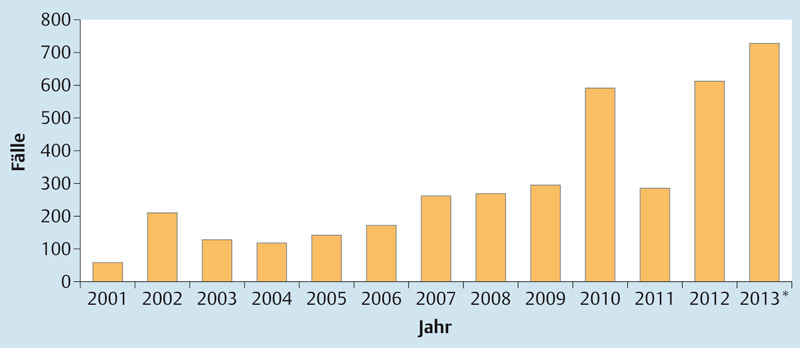
\includegraphics[scale=0.5]{Images/infektionszahlen_dengue_virus_deutschland.jpeg}
  \caption{Entwicklung der Infektionszahlen des Dengue-Virus von 2001 bis 2013. Die x-Achse zeigt die Jahre, w\"ahrend die y-Achse die Anzahl der gemeldeten F\"alle darstellt. Der h\"ochste Wert von etwa 750 F\"allen wird im Jahr 2013 erreicht, w\"ahrend der niedrigste Wert mit circa 50 F\"allen im Jahr 2001 verzeichnet wird. Diese Daten verdeutlichen den signifikanten Anstieg der Infektionen \"uber den betrachteten Zeitraum. Quelle: \citetitle{cramer_dengue-virus_2014} \cite{cramer_dengue-virus_2014}.}
  \label{fig:Dengue_virus_infektionszahlen_deutschland}
\end{figure} Dengue-Viren sind besonders geschickt darin, das menschliche Immunsystem zu \"uberlisten. Sie haben "`perfide Tricks"' entwickelt, um der Immunabwehr zu entgehen~\cite{janisch_klein_2017}. Die zunehmende Verbreitung von Dengue-Viren und deren Vektoren, also den Organismen, die das Virus \"ubertragen (in diesem Fall die Stechm\"ucken), stellt eine wachsende Herausforderung f\"ur das Gesundheitswesen dar, auch in Regionen, die traditionell nicht als Risikogebiete galten~\cite{cramer_dengue-virus_2014}. Es ist wichtig, die Mutationen der Virenfamilie zu untersuchen und Vorhersagen \"uber die Bereiche zu machen, wo das Virus stabil ist und wo Mutationen wahrscheinlich auftreten. Viren wie die Dengue-Viren sind Meister darin, das Immunsystem des Menschen zu \"uberlisten. Durch Mutationen k\"onnen sie sich besser an neue Wirte und Umgebungen anpassen, was ihre Verbreitung erleichtert und die Bek\"ampfung erschwert~\cite{cramer_dengue-virus_2014, janisch_klein_2017}. Das Verst\"andnis der Mutationsmuster hilft bei der epidemiologischen \"Uberwachung. Wenn bekannt ist, welche Bereiche des Virusgenoms stabil sind und welche zu Mutationen neigen, k\"onnen Gesundheitsbeh\"orden besser absch\"atzen, wann und wo neue Ausbr\"uche auftreten k\"onnten. Dies ist besonders wichtig in Regionen, in denen invasive Stechm\"uckenarten wie Aedes albopictus nachgewiesen wurden, die als Vektoren f\"ur verschiedene Viren dienen k\"onnen~\cite{cramer_dengue-virus_2014}. Die F\"ahigkeit, Mutationen vorherzusagen, kann helfen, potenzielle Pandemien fr\"uhzeitig zu erkennen und Ma\ss{}nahmen zu ergreifen, bevor sich das Virus weit verbreitet~\cite{janisch_klein_2017}. Durch die Identifikation stabiler und variabler Regionen des Virusgenoms k\"onnen stabilere Impfstoffe und gezieltere Therapien entwickelt werden. Bei der Entwicklung von Impfstoffen und Medikamenten ist es wichtig, absch\"atzen zu k\"onnen, welche Teile des Virus mutieren, da Impfstoffe und antivirale Therapien oft auf spezifische Teile des Virus zielen. Wenn diese Teile mutieren, k\"onnen Impfstoffe und Medikamente weniger wirksam werden~\cite{janisch_klein_2017}. 
Insgesamt erm\"oglicht die Untersuchung von Virusmutationen eine proaktive und gezielte Reaktion auf virale Bedrohungen, was entscheidend f\"ur den Schutz der \"offentlichen Gesundheit ist.

\section{Aufbau und Struktur der Arbeit}
In dieser Arbeit wird somit untersucht, inwieweit die Transmembranproteine des Dengue-Virus hinsichtlich Hydropathie und Polar-Requirement besonders konserviert sind. Um diese Fragestellung zu bearbeiten, gliedert sich die Arbeit in folgende Kapitel: Kapitel 1 bietet eine Einf\"uhrung in die biochemischen Grundlagen von Proteinen und das Dengue-Virus. Hierbei wird das notwendige Hintergrundwissen vermittelt, um das Verst\"andnis f\"ur die folgenden Analysen zu f\"ordern. Kapitel 2 beschreibt die verwendeten Materialien und Methoden, einschlie\ss{}lich der (bio-)chemischen und bioinformatischen Grundlagen und erkl\"art die zugrundeliegende Analyse des Dengue-Virus. Dieser Abschnitt ist entscheidend, um die Methodik zu verstehen, die zur Erhebung und Auswertung der Daten verwendet wurde. Kapitel 3 pr\"asentiert die Ergebnisse der durchgef\"uhrten Analysen. Kapitel 4 diskutiert die Ergebnisse im Kontext bestehender Literatur und zieht Schlussfolgerungen. Hierbei werden auch m\"ogliche Implikationen f\"ur zuk\"unftige Forschungen aufgezeigt. Kapitel 5 fasst die wichtigsten Erkenntnisse zusammen und gibt einen Ausblick auf zuk\"unftige Forschungsrichtungen.

\chapter{Material und Methoden}%: Document Setup and Document Structure}
\label{chapter-use}
In diesem Abschnitt werden die biochemischen und bioinformatischen Grundlagen beschrieben, die f\"ur die Analyse der Stabilit\"at von Transmembranproteinen des Dengue-Virus entscheidend sind. Um ein umfassendes Verst\"andnis f\"ur die Analyse von Transmembranproteinen zu entwickeln, ist es wichtig, sowohl die chemischen Grundlagen als auch die informatischen Methoden zu betrachten. Im ersten Teil dieses Kapitels werden die biochemischen Aspekte behandelt, insbesondere die spezifischen Eigenschaften des Dengue-Virus sowie die Konzepte der Hydropathie, die F\"ahigkeit von Aminos\"auren, sich in einer hydrophoben Umgebung zu verankern, und der Polar-Requirement, die quantifizieren, wie wichtig eine Aminos\"aure an ihrem spezifischen Platz im Protein ist. Diese Grundlagen sind entscheidend, um zu verstehen, wie das Virus aufgebaut ist und welche Rolle Hydropathie und Polar-Requirement bei der Mutationsanalyse spielen. Im zweiten Teil des Kapitels liegt der Fokus auf den bioinformatischen Methoden, die zur Analyse der gesammelten Daten verwendet werden. Hierbei werden verschiedene Schritte wie Datenerfassung, Datenstrukturierung, Datenausrichtung, Berechnung und Visualisierung erl\"autert. Diese Methoden sind unerl\"asslich, um die relevanten Informationen aus den biologischen Daten zu extrahieren und sie in einem verst\"andlichen Format darzustellen. 

\section{(Bio-)chemische Grundlagen}
In diesem Abschnitt werden die biochemischen Grundlagen behandelt, die f\"ur das Verst\"andnis der Transmembranproteine des Dengue-Virus von zentraler Bedeutung sind. Transmembranproteine spielen eine entscheidende Rolle in der Zellbiologie, da sie die Interaktion zwischen der Zelle und ihrer Umgebung erm\"oglichen. Insbesondere bei Virusproteinen wie denen des Dengue-Virus sind diese Eigenschaften von gro\ss{}er Bedeutung, da sie die Stabilit\"at und Funktionalit\"at der Proteine beeinflussen k\"onnen. Zun\"achst wird das Dengue-Virus vorgestellt, einschlie\ss{}lich seiner Struktur und der spezifischen Eigenschaften seiner Transmembranproteine. Diese Informationen sind wichtig, um die biologischen Funktionen des Virus zu verstehen und wie es mit Wirtszellen interagiert. Anschlie\ss{}end wird das Konzept der Hydropathie sowie die Polar-Requirement erl\"autert. Diese beiden Aspekte sind entscheidend f\"ur die Analyse der molekularen Eigenschaften von Proteinen, da sie Aufschluss dar\"uber geben, wie hydrophobe und hydrophile Bereiche innerhalb der Transmembranregionen wirken und welche Rolle sie bei der Stabilit\"at und Funktion der Proteine spielen. Durch das Verst\"andnis dieser biochemischen Grundlagen wird eine solide Basis geschaffen, um die folgenden bioinformatischen Methoden und deren Anwendung in der Analyse von Mutationsstabilit\"at zu er\"ortern.

\subsection{Dengue-Virus}
Dengue-Viren sind umh\"ullte, positiv-str\"angige RNA-Viren, die zur Familie der Flaviviridae geh\"oren. Diese Viren werden in vier Serotypen eingeteilt: DENV-1~\cite{tittarelli_dengue_2014}, DENV-2~\cite{cao_retrospective_2023}, DENV-3~\cite{peyrefitte_genetic_2003} und DENV-4~\cite{wardhani_genetic_2023}. Serotypen sind Untergruppen von Mikroorganismen, wie Viren oder Bakterien, die sich durch spezifische antigenetische Eigenschaften unterscheiden. Diese Unterschiede beziehen sich auf die Struktur von Antigenen, die auf der Oberfl\"ache der Mikroben vorhanden sind. Serotypen k\"onnen durch serologische Tests identifiziert werden, bei denen Antik\"orper verwendet werden, um die Reaktion auf bestimmte Antigene zu bestimmen. Der Virusk\"orper besteht aus einer Lipid-Doppelschicht, die von Membran- (M) und H\"ullproteinen (E) durchsetzt ist. Im Inneren befindet sich das Nukleokapsid, das aus dem Kapsidprotein (C) und dem Genom-RNA-Strang zusammengesetzt ist. Die H\"ullproteine (E) sind Typ-II-Transmembranproteine, die aus einer N-terminalen Ektodom\"ane, einer Transmembrandom\"ane und einer C-terminalen zytoplasmatischen Dom\"ane bestehen. Die Ektodom\"ane ist f\"ur die Bindung an Wirtszellrezeptoren und die Fusion mit der Wirtszellmembran verantwortlich. Die Transmembrandom\"ane verankert das E-Protein in der Virush\"ulle und durchspannt die Lipid-Doppelschicht. Die kurze zytoplasmatische Dom\"ane interagiert mit dem Kapsidprotein. Die Membranproteine (M) sind ebenfalls Typ-II-Transmembranproteine, die aus einer N-terminalen Ektodom\"ane, einer Transmembrandom\"ane und einer C-terminalen zytoplasmatischen Dom\"ane aufgebaut sind. Sie sind an der Reifung und Freisetzung infekti\"oser Viruspartikel beteiligt und sind damit die strukturellen Proteine des Virus. Beide Transmembranproteine, E und M, durchspannen die Lipid-Doppelschicht der Virush\"ulle mit ihren hydrophoben Transmembrandom\"anen. Diese Dom\"anen sind f\"ur die Verankerung und Stabilit\"at der Proteine in der Membran von entscheidender Bedeutung. Mutationen in diesen Regionen k\"onnen die Faltung, Insertion und Stabilit\"at der Proteine beeinflussen und somit die Infektiosit\"at und \"Uberlebensf\"ahigkeit des Virus beeintr\"achtigen. Weiterhin besitzt das Dengue-Virus ein Signalpeptid "`2K"'. 2K ist ein kleines Protein, das als Transmembranprotein fungiert und eine Rolle bei der Virusreifung spielt. Dengue-Viren besitzen au\ss{}erdem sieben nicht-strukturelle Proteine, die f\"ur den Lebenszyklus des Virus entscheidend sind: NS1, NS2A, NS2B, NS3, NS4A, NS4B und NS5. NS1 ist ein wichtiges virales Glykoprotein, das in der Zelle sekretiert wird und an der Virusreplikation beteiligt ist. Es hat keine transmembrane Region, sondern ist haupts\"achlich im Zytoplasma und im Extrazellularraum aktiv. NS2A ist ein kleines, hydrophobes Protein, das als Transmembranprotein wirkt und an der Membran des endoplasmatischen Retikulums lokalisiert ist. Es spielt eine Rolle bei der Virusreplikation und der Modifikation der Wirtszellmembran. NS2B ist ein Co-Faktor f\"ur die Protease NS3 und hat eine transmembrane Region, die es in die Membran des endoplasmatischen Retikulums einbettet. NS3 ist ein wichtiges Enzym, das als Serinprotease und RNA-Helikase fungiert und dadurch eine entscheidende Rolle bei der Virusreplikation spielt, indem es das Polyprotein nach der Synthetisierung spaltet und die virale RNA entwindet. Es hat eine transmembrane Region, die es in die Membran integriert. NS4A ist ebenfalls ein Transmembranprotein und spielt eine Rolle in der Virusreplikation und der Modulation der Wirtszellantwort. NS4B ist ein weiteres Transmembranprotein, das an der Virusreplikation beteiligt ist und in der Membran des endoplasmatischen Retikulums lokalisiert ist. NS5 ist das gr\"o\ss{}te Protein des Dengue-Virus, das als RNA-abh\"angige RNA-Polymerase fungiert und somit f\"ur die Vervielf\"altigung des viralen Genoms verantwortlich ist. Es hat auch eine transmembrane Region, die es in die Membran einbettet.
Insgesamt sind die Transmembranproteine im Dengue-Virus: E, M, 2K, NS2A, NS2B, NS3, NS4A, NS4B und NS5. Wobei NS2A fast vollst\"andig in der Membran verankert liegt. Der Aufbau des Dengue-Virus und die transmembranen Regionen sind in der Abbildung \ref{fig:Dengue_virus_overview} aus dem Paper \citetitle{perera_structural_2008} von \citeauthor{perera_structural_2008}~\cite{perera_structural_2008} visualisiert. 
\begin{figure}[tbp]
  \centering
  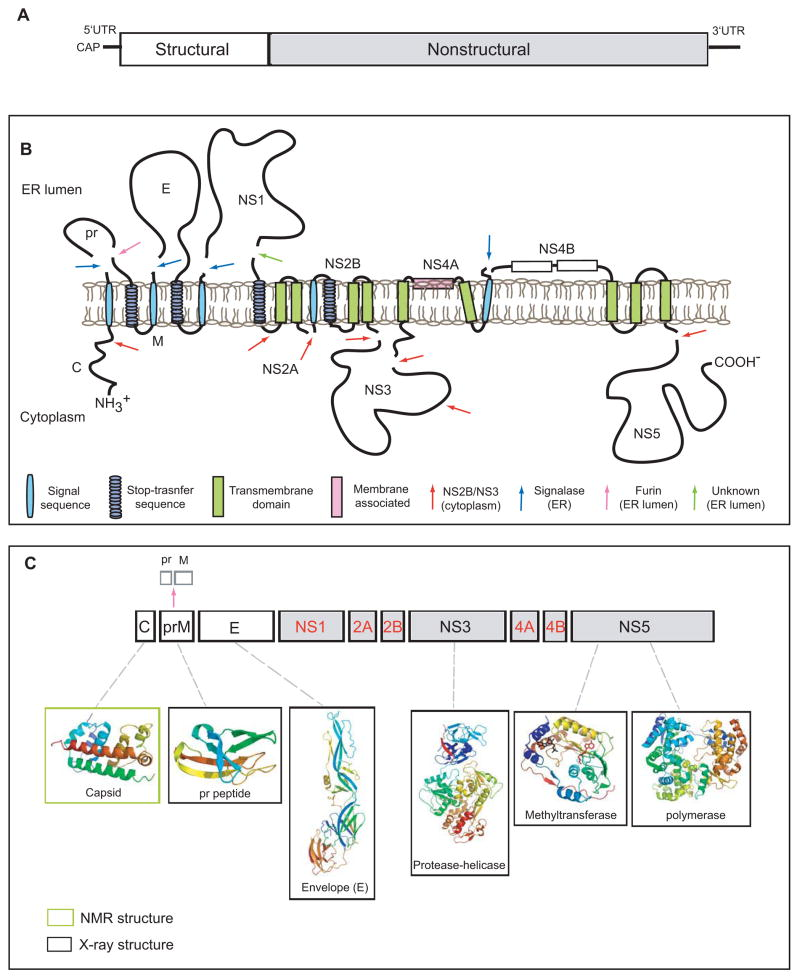
\includegraphics[scale=1]{Images/Dengue_virus_overview.jpg}
  \caption{Visualisierung des Aufbaus des Dengue-Virus und seiner transmembranalen Regionen. Die Abbildung zeigt die Struktur des Virus sowie die Anordnung der verschiedenen Proteine. Diese Darstellung basiert auf den Ergebnissen von \citeauthor{perera_structural_2008} und bietet Einblicke in die strukturellen Eigenschaften der Transmembranproteine des Dengue-Virus. Quelle: \citetitle{perera_structural_2008} \cite{perera_structural_2008}.}
  \label{fig:Dengue_virus_overview}
\end{figure} 

Die Untersuchung der Transmembranproteine im Dengue-Virus bietet nicht nur Einblicke in deren strukturelle Eigenschaften, sondern \"offnet auch den Weg zu einem tiefergehenden Verst\"andnis der Wechselwirkungen zwischen diesen Proteinen und ihrer Umgebung. Insbesondere die hydrophoben und hydrophilen Bereiche der Transmembranregionen spielen eine entscheidende Rolle f\"ur die Stabilit\"at und Funktionalit\"at der Proteine. Um die spezifischen Eigenschaften dieser Bereiche zu quantifizieren, ist es notwendig, die Konzepte der Polar-Requirement und der Hydropathie zu betrachten. Diese Konzepte erm\"oglichen es, die hydrophilen und hydrophoben Eigenschaften der Aminos\"auresequenzen zu messen und zu analysieren, was f\"ur das Verst\"andnis der Interaktionen zwischen den transmembran Bereichen und ihrer Umgebung von zentraler Bedeutung ist.

\subsection{Hydropathie und Polar-Requirement}
Hydropathie beschreibt die Affinit\"at eines Molek\"uls zu Wasser und klassifiziert Molek\"ule als hydrophil (wasserliebend) oder hydrophob (wasserabweisend). Diese Eigenschaften beeinflussen, wie Molek\"ule in biologischen Systemen interagieren, insbesondere in Bezug auf Proteine und deren Funktion. Hydropathie wird besonders h\"aufig verwendet, um eine bestimmte Untergruppe von Proteinen, die Membranproteine, zu untersuchen. Diese Proteine k\"onnen transmembrane Regionen besitzen, in denen sie die Membran vollst\"andig durchdringen. Jedes Molek\"ul hat ein charakteristisches Hydropathie-Profil, das als eine Art "`Fingerabdruck"' f\"ur seine Struktur betrachtet werden kann. Diese Profile werden h\"aufig verwendet, um die Struktur und Funktion von Membranproteinen zu analysieren und um Beziehungen zwischen verschiedenen Transportproteinen zu identifizieren. In biologischen Systemen spielen hydrophobe und hydrophile Wechselwirkungen eine entscheidende Rolle bei der Faltung von Proteinen, der Bildung von Zellmembranen und der Funktion von Enzymen. Das Verst\"andnis dieser Eigenschaften hilft bei der Vorhersage, wie Molek\"ule in zellul\"aren Umgebungen interagieren. Hydropathie-Analysen werden in der Bioinformatik und Strukturbiologie eingesetzt, um die Topologie von Membranproteinen vorherzusagen und deren funktionelle Eigenschaften besser zu verstehen. Zusammenfassend ist die Hydropathie eine grundlegende chemische Eigenschaft, die entscheidend f\"ur das Verst\"andnis der Molek\"ulinteraktionen in biologischen Systemen ist, da sie die grundlegenden Molek\"uleigenschaften des Proteins beschreibt. Jede Aminos\"aure hat einen spezifischen Hydropathiewert. In dieser Arbeit verwenden wir die Werte aus dem Paper \citetitle{kyte_simple_1982} von \citeauthor{kyte_simple_1982}~\cite{kyte_simple_1982}, die in der Abbildung \ref{fig:Hydropathieindexe} dargestellt sind. Die Hydropathie-Indizes, wie sie von \citeauthor{kyte_simple_1982} entwickelt wurden, quantifizieren die hydrophoben und hydrophilen Eigenschaften von Aminos\"auren in Proteinen. Diese Indizes basieren auf der Messung der Energie, die erforderlich ist, um eine Aminos\"aure aus einer w\"assrigen L\"osung in eine hydrophobe Umgebung zu transferieren. F\"ur jede Aminos\"aure wurde ein Wert zugewiesen, der ihre Neigung beschreibt, sich in w\"assriger Umgebung zu l\"osen oder in einer hydrophoben Phase zu verbleiben. Die Werte reichen von stark negativ (sehr hydrophil) bis stark positiv (sehr hydrophob).
\begin{figure}[tbp]
  \centering
  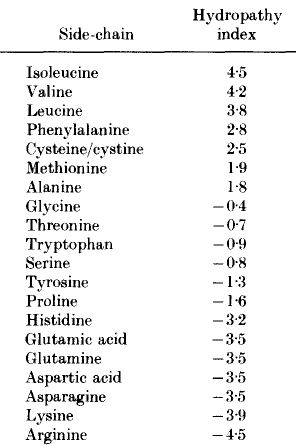
\includegraphics[scale=0.75]{Images/Hydropathy_scores_Paper.png}
  \caption{Tabelle der Aminos\"auren mit den zugeh\"origen Hydropathie-Indizes. Die Werte basieren auf den Ergebnissen von \citeauthor{kyte_simple_1982} und dienen als Grundlage f\"ur die Analyse der hydrophoben und hydrophilen Eigenschaften von Aminos\"auren in den Transmembranproteinen des Dengue-Virus. Diese Indizes sind entscheidend f\"ur das Verst\"andnis der Interaktionen zwischen den Aminos\"auren und ihrer Umgebung. Quelle: \citetitle{kyte_simple_1982} \cite{kyte_simple_1982}.}
  \label{fig:Hydropathieindexe}
\end{figure}
In dem Paper \citetitle{kyte_simple_1982}~\cite{kyte_simple_1982} werden vier spezifische Werte des Hydropathie-Index manuell angepasst. Diese Anpassungen betreffen die Aminos\"auren Glycin, Alanin, Serin und Threonin. Diese Anpassungen wurden vorgenommen, um die Hydropathie-Indizes dieser Aminos\"auren so zu modifizieren, dass sie besser die experimentellen Beobachtungen und biologischen Eigenschaften der Proteine widerspiegeln.

Im chemischen Kontext beziehen sich "`Polar-Requirement"' auf die spezifischen Eigenschaften und Bedingungen, die f\"ur polare Molek\"ule oder chemische Verbindungen erforderlich sind, um in einer bestimmten Umgebung stabil zu sein oder zu interagieren. Diese Anforderungen k\"onnen die Polarit\"at, L\"oslichkeit, Wechselwirkungen mit anderen Molek\"ulen und die F\"ahigkeit zur Bildung von Wasserstoffbr\"ucken umfassen. Molek\"ule mit polaren Gruppen (z. B. Hydroxyl- oder Carboxylgruppen) haben unterschiedliche Eigenschaften im Vergleich zu unpolaren Molek\"ulen. Die Polarit\"at beeinflusst, wie Molek\"ule in L\"osungsmitteln interagieren, insbesondere in w\"assrigen L\"osungen. Polare Molek\"ule sind in polaren L\"osungsmitteln wie Wasser besser l\"oslich. Die Polar-Requirement helfen zu bestimmen, welche Molek\"ule in bestimmten chemischen Reaktionen oder biologischen Prozessen effektiv interagieren k\"onnen. Die Polar-Requirement sind entscheidend f\"ur die Vorhersage von Wechselwirkungen zwischen Molek\"ulen, wie z. B. zwischen Enzymen und Substraten oder zwischen Rezeptoren und Liganden. In der Biochemie sind die Polar-Requirement wichtig f\"ur das Verst\"andnis der Struktur und Funktion von Biomolek\"ulen, einschlie\ss{}lich Proteinen und Nukleins\"auren. Auch Polar-Requirement sind entscheidend f\"ur das grundlegende Verst\"andnis der Molek\"uleigenschaften eines Proteins. 
Aminos\"auren haben spezifische Polar-Requirement-Werte. In dieser Arbeit nutzen wir die Werte aus der Arbeit \citetitle{woese_fundamental_1966} von \citeauthor{woese_fundamental_1966}~\cite{woese_fundamental_1966}, die in der Abbildung \ref{fig:Polar_requirements_indexe} dargestellt sind. 
\begin{figure}[tbp]
  \centering
  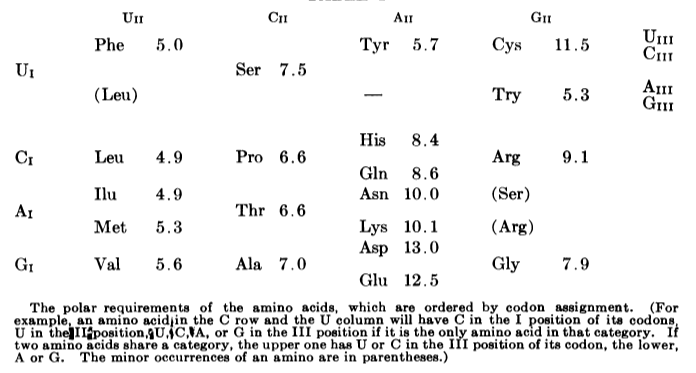
\includegraphics[scale=0.6]{Images/polar_requirements_scores_Paper.png}
  \caption{Tabelle der Aminos\"auren mit den zugeh\"origen Polar-Requirement-Werten. Die Werte basieren auf den Ergebnissen von \citeauthor{woese_fundamental_1966} und dienen als Grundlage f\"ur die Analyse der polarisierten Eigenschaften von Aminos\"auren in den Transmembranproteinen des Dengue-Virus. Diese Indizes sind entscheidend f\"ur das Verst\"andnis der Interaktionen zwischen den Aminos\"auren und ihrer Umgebung. Quelle: \citetitle{woese_fundamental_1966} \cite{woese_fundamental_1966}.}
  \label{fig:Polar_requirements_indexe}
\end{figure}
Dabei ist zu beachten, dass der Cysteinwert von 11,5 auf 5,5, in dem Paper \citetitle{woese_evolution_1973} von \citeauthor{woese_evolution_1973} im Jahr \citeyear{woese_evolution_1973}~\cite{woese_evolution_1973}, korrigiert wurde, um die hydrophobe Natur der Aminos\"aure Cystein genauer darzustellen. Wir nutzen somit die Tabelle mit einem angepassten Cysteinwert von 5,5. 
Die Polar-Requirement-Werte, wie sie von \citeauthor{woese_fundamental_1966} eingef\"uhrt wurden, geben an, wie stark eine Aminos\"aure polare Wechselwirkungen eingeht. Diese Werte wurden durch die Messung der freien Enthalpie berechnet, die erforderlich ist, um eine Aminos\"aure von einer unpolaren in eine polare Umgebung zu transferieren. Die Polar-Requirement-Werte wurden in einem Experiment bestimmt, bei dem die L\"oslichkeit jeder Aminos\"aure in Wasser und einem unpolaren L\"osungsmittel gemessen wurde. Konkret wurde Octanol als unpolare Phase verwendet. Das Experiment lief folgenderma\ss{}en ab: F\"ur jede der 20 proteinogenen Aminos\"auren wurde die L\"oslichkeit in Wasser und Octanol bestimmt. Dazu wurde eine definierte Menge der Aminos\"aure in beide L\"osungsmittel gegeben und die Konzentration in der jeweiligen Phase gemessen. Aus dem Unterschied in der L\"oslichkeit konnte dann die freie Enthalpie f\"ur den Transfer zwischen den beiden Phasen berechnet werden. Je gr\"o\ss{}er der Wert, desto st\"arker die Tendenz der Aminos\"aure, polare Wechselwirkungen einzugehen und sich in einer w\"assrigen Umgebung aufzuhalten. Die Werte reichen von sehr niedrig (unpolar) bis sehr hoch (polar). Sie erm\"oglichen es, die Aminos\"auren nach ihrer Polarit\"at zu ordnen und R\"uckschl\"usse auf die Oberfl\"achenexposition und Interaktionen von Proteinen zu ziehen. In Kombination mit anderen Parametern wie den Hydropathie-Indizes liefern sie wertvolle Informationen f\"ur die Strukturvorhersage und das Proteindesign. Diese hydrophoben und hydrophilen Eigenschaften sind entscheidend f\"ur das Verst\"andnis der funktionalen Regionen von Proteinen, insbesondere in Bezug auf die Stabilit\"at der Transmembranregionen im Dengue-Virus. Die Analyse der Hydropathie-Indizes und der Polar-Requirment-Werte erm\"oglicht es uns, spezifische Bereiche innerhalb des Genoms (Abbildung \ref{fig:Dengue_virus_overview}) zu identifizieren, die voraussichtlich st\"arker konserviert sind. Diese Bereiche k\"onnten entscheidend f\"ur die Funktionalit\"at der Proteine sein und helfen, die Mutationsstabilit\"at besser zu verstehen. Es sollte somit anhand der Werte in den jeweiligen Regionen erkennbar sein, in welchen Bereichen st\"arker konservierte Transmembranproteine liegen.

Obwohl Hydropathie und Polar-Requirement \"ahnliche Eigenschaften untersuchen, zeigt sich bei den Werten einige Unterschiede. Da nicht alle Aminos\"auren eindeutig zu klassifizieren sind, wenn man nur eine der beiden Molek\"uleigenschaften verwendet und somit wertvolle Informationen \"uber die Struktur des Proteins verloren geht. Aus diesem Grund verwenden wir beide Werte f\"ur die Berechnung. 

\section{(Bio-)informatische Grundlagen}
\begin{figure}[tbp]
    \centering
    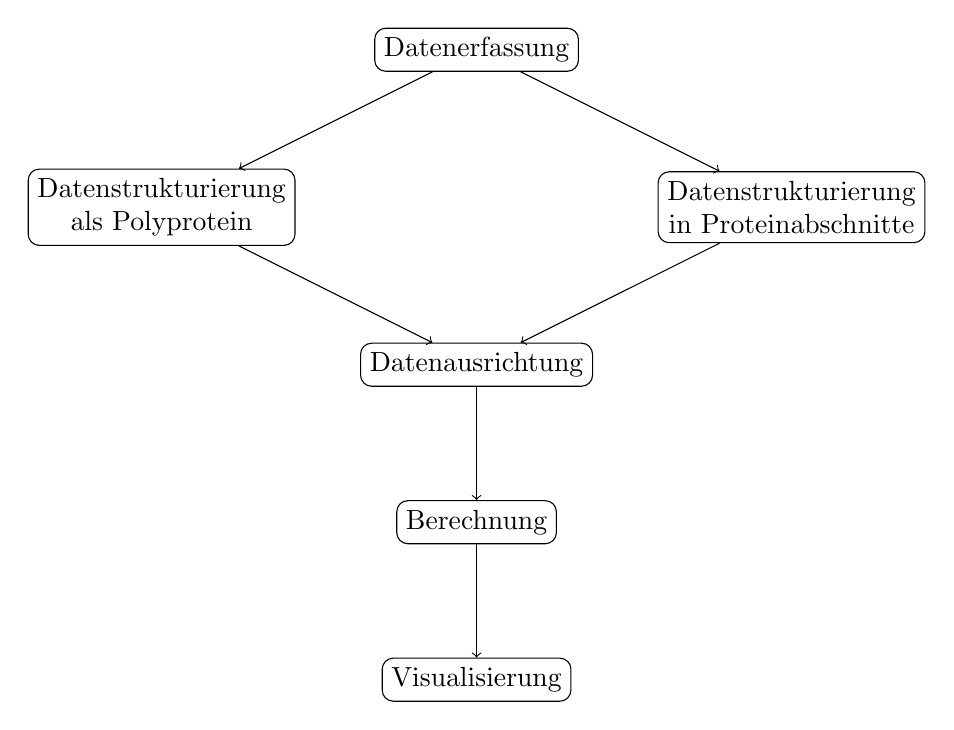
\begin{tikzpicture}
    \node (start) [rectangle, rounded corners, draw] at (0, 0) {Datenerfassung};
    \node (strukt1) [rectangle, rounded corners, draw, align=center] at (-4, -2) {Datenstrukturierung \\ als Polyprotein};
    \node (strukt2) [rectangle, rounded corners, draw, align=center] at (4, -2) {Datenstrukturierung \\ in Proteinabschnitte};
    \node (align) [rectangle, rounded corners, draw] at (0, -4) {Datenausrichtung};
    \node (calc) [rectangle, rounded corners, draw] at (0, -6) {Berechnung};
    \node (vis) [rectangle, rounded corners, draw] at (0, -8) {Visualisierung};

    % Zeichne die Pfeile
    \draw[->] (start) -- (strukt1);
    \draw[->] (start) -- (strukt2);
    \draw[->] (strukt1) -- (align);
    \draw[->] (strukt2) -- (align);
    \draw[->] (align) -- (calc);
    \draw[->] (calc) -- (vis);
    \end{tikzpicture}
    \caption{Visualisierung des Datenverarbeitungsprozesses}
    \caption{Visualisierung des Datenverarbeitungsprozesses zur Analyse der Stabilit\"at von Transmembranproteinen. Der Prozess beginnt mit der Datenerfassung, gefolgt von der Datenstrukturierung sowohl als Polyprotein als auch in einzelne Proteinabschnitte. Nach der Datenausrichtung erfolgt die Berechnung, bevor die Ergebnisse schlie\ss{}lich visualisiert werden. Diese Abbildung veranschaulicht die einzelnen Schritte und deren Zusammenh\"ange im Rahmen der bioinformatischen Analyse.}
    \label{fig:datenverarbeitung}
\end{figure} 

In diesem Abschnitt werden die bioinformatischen Grundlagen behandelt, die f\"ur die Analyse der Stabilit\"at von Transmembranproteinen und deren Mutationsverhalten entscheidend sind. Die Verarbeitung biologischer Daten ist ein wesentlicher Bestandteil der modernen biomedizinischen Forschung, insbesondere wenn es darum geht, komplexe molekulare Interaktionen zu verstehen. Die Datenverarbeitung wird in der Abbildung \ref{fig:datenverarbeitung} visualisiert. Der erste Schritt in diesem Prozess ist die Datenerfassung. Anschlie\ss{}end erfolgt die Datenstrukturierung, um die gesammelten Informationen in ein geeignetes Format zu bringen. Nach der Strukturierung werden die Daten ausgerichtet, was es erlaubt, Sequenzen zu vergleichen. Im Anschluss daran erfolgt die Berechnung. Schlie\ss{}lich werden die Ergebnisse visualisiert. In den folgenden Abschnitten werden diese Schritte im Detail erl\"autert, um ein umfassendes Verst\"andnis f\"ur die bioinformatischen Methoden zu vermitteln, die in dieser Arbeit verwendet werden.

\subsection{Datenerfassung}
F\"ur die Datenverarbeitung werden FASTA-Dateien als Eingabe ben\"otigt. Das FASTA-Dateiformat ist ein textbasiertes Format zur Darstellung von Nukleotid- oder Proteinsequenzen und erm\"oglicht die Speicherung mehrerer Sequenzen in einer einzigen Datei. Um die Daten f\"ur die Berechnung zu erstellen, wurden FASTA-Daten von allen Dengue-Virus-Serotypen (DENV-1~\cite{tittarelli_dengue_2014}, DENV-2~\cite{cao_retrospective_2023}, DENV-3~\cite{peyrefitte_genetic_2003} und DENV-4~\cite{wardhani_genetic_2023}) aus GenBank~\cite{genbank} genutzt. GenBank ist eine der bedeutendsten Datenbanken f\"ur DNA-Sequenzen und wird vom National Center for Biotechnology Information (NCBI) betrieben. Sie enth\"alt \"uber 240 Millionen Sequenzen von mehr als einer Million Spezies und dient als zentrale Ressource f\"ur Wissenschaftler, um genetische Informationen zu speichern, abzurufen und zu analysieren. Die Verwendung von GenBank-Daten erm\"oglicht es, umfassende und aktuelle Informationen \"uber die verschiedenen Serotypen des Dengue-Virus zu erhalten. Diese Daten sind entscheidend f\"ur die anschlie\ss{}enden bioinformatischen Analysen, da sie die Grundlage f\"ur die Untersuchung der Mutationsstabilit\"at und der strukturellen Eigenschaften der Transmembranproteine bilden.

\subsection{Datenstrukturierung}
Die einzelnen FASTA-Daten k\"onnen auf zwei verschiedenen Arten strukturiert werden. Entweder werden alle vier DNA-Sequenzen der vier Serotypen in einer einzigen FASTA-Datei gespeichert, wodurch das gesamte Polyprotein f\"ur die nachfolgende Berechnung genutzt wird, oder die Sequenzen werden in die einzelnen Proteinabschnitte unterteilt, um spezifische Aussagen \"uber die einzelnen Proteine treffen zu k\"onnen. F\"ur die zweite Variante werden GenPept-Daten aus GenBank ben\"otigt. GenPept ist ein Datenformat, das Annotationen speichert, wie z.B. die Positionen der Proteine innerhalb der Sequenzen. Diese Daten k\"onnen genau wie die FASTA-Daten aus GenBank geladen werden. In dieser Arbeit wurde f\"ur ein Programm in Python~\cite{python} entwickelt, das jeweils einen GenPept-Datensatz eines Serotypen als Eingabe erh\"alt und diese Datei mithilfe von den Biopython-Modulen~\cite{cock2009biopython} SeqIO und SeqRecord, sowie Path aus pathlib~\cite{pathlib} in einen Ordner strukturiert speichert. F\"ur jedes annotierte Protein wird eine eigene FASTA-Datei erstellt. Mit SeqIO wird dabei die DNA-Sequenz aus der GenPept-Datei gelesen und in die neue FASTA-Datei geschrieben. SeqRecord wird benutzt, um die Kopfzeile der FASTA-Datei zu formatieren und dort unter anderem den Namen des Proteins einzutragen. Pathlib wird anschlie\ss{}end verwendet, um die neuen FASTA-Dateien in einem Ordner zu sammeln und zu speichern, um den Zugriff und die Zuordnung zu dem jeweiligen Serotypen zu erleichtern. F\"ur jeden Serotyp wird ein separater Ordner erstellt, in dem jedes Protein in einer eigenen FASTA-Datei abgespeichert ist. Zuletzt m\"ussen die vier Ordner manuell zusammengef\"uhrt werden, indem jedes Protein in jedem der vier Ordner gesucht und in einer gemeinsamen FASTA-Datei gespeichert wird. Am Ende existiert ein gemeinsamer Ordner, in dem jedes Protein eine eigene FASTA-Datei mit den vier DNA-Str\"angen der verschiedenen Serotypen enth\"alt.

\subsection{Datenausrichtung}
Um die Daten auszurichten, werden die zuvor strukturierten FASTA-Daten einzeln manuell in das Online-Tool T-Coffee~\cite{tcoffee} eingegeben. Die Ausgabe wird auf das FASTA-Dateiformat eingestellt, sodass wir im Folgenden mit ausgerichteten FASTA-Dateien als Eingabe weiterarbeiten k\"onnen. T-Coffee (Tree-based Consistency Objective Function for Alignment Evaluation) ist ein in der Bioinformatik weit verbreitetes Werkzeug zur Ausrichtung von DNA-, RNA- und Proteinsequenzen. T-Coffee arbeitet mit einer Ausrichtungsstrategie in Kombination mit einer konsistenzbasierten Bewertungsfunktion. Der Algorithmus f\"ur T-Coffee wird haupts\"achlich in der Originalver\"offentlichung \citetitle{poirot_tcoffeeigs_2003}~\cite{poirot_tcoffeeigs_2003} beschrieben. Der Algorithmus hat die folgenden Hauptschritte. Zun\"achst generiert T-Coffee alle m\"oglichen paarweisen Ausrichtungen zwischen den Eingabesequenzen unter Verwendung globaler und lokaler Ausrichtungsmethoden. Anschlie\ss{}end erstellt es eine prim\"are Bibliothek mit Ausrichtungsinformationen aus diesen paarweisen Ausrichtungen und weist jedem ausgerichteten Residuenpaar basierend auf seiner Konsistenz \"uber verschiedene Ausrichtungen hinweg Gewichte zu. Die prim\"are Bibliothek wird durch Einbeziehung transitiver Ausrichtungen erweitert, was hilft, indirekte Beziehungen zwischen Sequenzen zu erfassen. Unter Verwendung der erweiterten Bibliothek konstruiert T-Coffee einen F\"uhrungsbaum und f\"uhrt eine progressive Ausrichtung durch, bei der zun\"achst die \"ahnlichsten Sequenzen ausgerichtet und dann nach und nach entferntere Sequenzen hinzugef\"ugt werden. Die anf\"angliche Ausrichtung wird iterativ verfeinert, um ihre Gesamtqualit\"at und -konsistenz zu verbessern. T-Coffee zeichnet sich durch seine hohe Genauigkeit aus, insbesondere bei der Bearbeitung kurzer Sequenzen. In Vergleichsstudien hat es gezeigt, dass es Ausrichtungen mit einer Genauigkeit produziert, die mit anderen Methoden wie MUSCLE~\cite{Edgar2004MUSCLEL} vergleichbar oder besser ist.

\subsection{Berechnung}
In diesem Abschnitt werden die Berechnungen zur Analyse der Mutationen im Polyprotein des Dengue-Virus beschrieben. Diese Berechnungen wurden in Python implementiert, wobei das SeqIO-Modul der Biopython-Bibliothek verwendet wurde, um die Sequenzen aus einer FASTA-Datei zu lesen und zu verarbeiten. Die Ergebnisse dieser Berechnungen werden im Anschluss detailliert vorgestellt.

F\"ur die Berechnung betrachten wir zun\"achst das Polyprotein des Dengue-Virus als Ganzes. Um die Ergebnisse zu berechnen, wurden die vier Sequenzen im Folgenden in 20 gleich gro\ss{}e Abschnitte aufgeteilt. F\"ur diese Abschnitte f\"uhren wir die Berechnungen einzeln durch, sodass wir f\"ur jeden Abschnitt ein Ergebnis erhalten, was am Ende einen Datenpunkt in einer Abbildung darstellt (siehe Ergebnisse). Da die Serotypen zuvor mit T-Coffee ausgerichtet wurden, sind alle Sequenzen gleich lang und k\"onnen somit in gleich gro\ss{}e Bereiche aufgeteilt werden. Im Folgenden wird von einzelnen Stellen der Sequenzen gesprochen; dabei ist gemeint, dass in der Ausrichtung an einer Stelle alle Sequenzen betrachtet werden.

Um den Anteil der Mutationen in einem Sequenzabschnitt zu quantifizieren, verwenden wir folgende Formel: 
\begin{equation}
    \text{Mutationsanteil} = \frac{\text{Anzahl der Positionen mit Mutationen}}{\text{Gesamtl\"ange des Sequenzabschnitts}} \label{eq:Anteil_an_Mutationen}
\end{equation}
Hierbei z\"ahlen wir als "`Positionen mit Mutationen"' alle Stellen, an denen wir mindestens zwei verschiedene Aminos\"auren oder eine L\"ucke vorfinden. Die "`Gesamtl\"ange des Sequenzabschnitts"' entspricht der Anzahl der betrachteten Positionen.

F\"ur die Berechnung des Polar-Requirement-Wertes einer Teilsequenz gehen wir wie folgt vor. Zuerst ermitteln wir f\"ur jede Position in der Teilsequenz den minimalen ($PR_{\text{min},i}$) und maximalen ($PR_{\text{max},i}$) Polar-Requirement-Wert der dort vorkommenden Aminos\"auren. Wir nutzen hierf\"ur die Werte aus der Abbildung \ref{fig:Polar_requirements_indexe} als Grundlage, um den Aminos\"auren Werte zuzuordnen, wobei wir die Werte auf einen Wertebereich zwischen 0 und 1 normieren. L\"ucken haben keine zugeordneten Werte und werden somit bei der Berechnung der Polar-Requirement nicht ber\"ucksichtigt, obwohl sie in der Berechnung f\"ur den Anteil der Mutationen gez\"ahlt werden. Details zu dieser Entscheidung werden im Kapitel Diskussion er\"ortert. Wir berechnen die Differenz zwischen dem maximalen und minimalen Wert an der jeweiligen Stelle und summieren diese Differenzen \"uber die gesamte L\"ange der Teilsequenz auf. Der finale Polar-Requirement-Wert ($PR_{\text{seq}}$) f\"ur die Teilsequenz ergibt sich aus dem Durchschnitt dieser Differenzen:
\begin{equation}
    PR_{\text{seq}} = \frac{1}{L} \sum_{i=1}^{L} (PR_{\text{max},i} - PR_{\text{min},i})
    \label{eq:polar_requirements}
\end{equation}
Hierbei ist $L$ die L\"ange der Teilsequenz und $i$ der Index der jeweiligen Position. Der resultierende $PR_{seq}$-Wert repr\"asentiert die durchschnittliche Variabilit\"at der Polar-Requirement-Werte innerhalb der Teilsequenz und liegt aufgrund der Normierung zwischen 0 (keine Variabilit\"at) und 1 (maximale Variabilit\"at).


F\"ur die Berechnung der Hydropathiewerte einer Teilsequenz gehen wir gleicherma\ss{}en vor. Zun\"achst ermitteln wir f\"ur jede Position in der Teilsequenz den minimalen ($H_{\text{min},i}$) und maximalen ($H_{\text{max},i}$) Hydropathiewert der dort vorkommenden Aminos\"auren. Hierf\"ur nutzen wir die Werte aus Abbildung \ref{fig:Hydropathieindexe} als Grundlage, wobei wir sicherstellen, dass diese Werte vorher auf einen Bereich zwischen 0 und 1 normiert werden. L\"ucken werden auch hier nicht ber\"ucksichtigt. Wir berechnen die Differenz zwischen dem maximalen und minimalen Wert an der jeweiligen Stelle und summieren diese Differenzen \"uber die gesamte L\"ange der Teilsequenz auf. Der finale Hydropathiewert ($H_{\text{seq}}$) f\"ur die Teilsequenz ergibt sich aus dem Durchschnitt dieser Differenzen:
\begin{equation}
    H_{\text{seq}} = \frac{1}{L} \sum_{i=1}^{L} (H_{\text{max},i} - H_{\text{min},i})
    \label{eq:hydropathie}
\end{equation} 
Hierbei ist $L$ wieder die L\"ange der Teilsequenz und $i$ der Index der jeweiligen Position. Der resultierende $H_{\text{seq}}$-Wert repr\"asentiert die durchschnittliche Variabilit\"at der Hydropathiewerte innerhalb der Teilsequenz und liegt aufgrund der Normierung zwischen 0 (keine Variabilit\"at) und 1 (maximale Variabilit\"at).

Um einen gemeinsamen Score zu bilden, welcher im Folgenden als "`Mutationsscore"' bezeichnet wird, werden die Werte f\"ur Polar-Requirement und Hydropathie f\"ur eine Teilsequenz gemittelt. Der Mutationsscore ($MS$) ergibt sich somit aus dem Durchschnitt der durchschnittlichen Variabilit\"at der Polar-Requirement-Werte sowie der durchschnittlichen Variabilit\"at der Hydropathie-Werte innerhalb einer Teilsequenz: 
\begin{equation}
    MS = \frac{1}{2} \left( PR_{\text{seq}} + H_{\text{seq}} \right)
    \label{eq:mutationsscore}
\end{equation}
Hierbei ist $PR_{\text{seq}}$ die durchschnittliche Variabilit\"at der Polar-Requirement-Werte und $H_{\text{seq}}$ die durchschnittliche Variabilit\"at der Hydropathie-Werte f\"ur die Teilsequenz. Der resultierende Mutationsscore stellt eine integrierte Bewertung der Variabilit\"at in Bezug auf Polar-Requirement und Hydropathie dar.

Zus\"atzlich wird die Berechnung des Mutationsscores gem\"a\ss{} Gleichung \ref{eq:mutationsscore} und der Anteile der Mutationen gem\"a\ss{} Gleichung \ref{eq:Anteil_an_Mutationen} erneut durchgef\"uhrt; jedoch nicht mit dem Polyprotein des Dengue-Virus in seiner urspr\"unglichen Form, sondern mit einer modifizierten Version, bei welcher die Sequenzen eine neue zuf\"allige Permutation aufweisen. Wir erstellen diese zuf\"allige Permutation des Dengue-Virus, indem wir eine Stelle in der Ausrichtung aller Serotypen zuf\"allig ausw\"ahlen und mit einer anderen zuf\"alligen Stelle vertauschen. Die allgemeine Ausrichtung bleibt dabei erhalten; es werden lediglich einzelne Positionen vertauscht. F\"ur die Abbildung \ref{fig:Dengue_virus_scores_and_mutations_bereiche_random}, welche in den Ergebnissen zu finden ist, wurden 10.000 zuf\"allige Vertauschungen nacheinander durchgef\"uhrt, sodass es m\"oglich ist, dass eine Stelle mehrfach vertauscht wird.

Zuletzt wird erneut die Berechnung des Mutationsscores gem\"a\ss{} Gleichung \ref{eq:mutationsscore} und dem Anteil der Mutationen gem\"a\ss{} Gleichung \ref{eq:Anteil_an_Mutationen} durchgef\"uhrt; diesmal jedoch unter Verwendung der zweiten Datenstrukturierung, bei welcher die Proteine f\"ur die Berechnung als Abschnitte verwendet werden, w\"ahrend bei den bisherigen Berechnungen gleich gro\ss{}e Bereiche ausgew\"ahlt wurden. Nun wird also f\"ur jedes Protein des Dengue-Virus ein Mutationsscore und ein Anteil an Mutationen berechnet.

\subsection{Visualisierung}
Um die Ergebnisse der Berechnungen zu visualisieren, wurden Abbildungen mithilfe der Bibliothek Matplotlib~\cite{matplotlib} erzeugt. F\"ur jeden Graphen wurde der jeweilige Durchschnittswert unter Verwendung von NumPy~\cite{numpy} berechnet. Diese Visualisierungen sind entscheidend, um die gewonnenen Daten anschaulich darzustellen und Muster sowie Trends in den Mutationsanalysen der Transmembranproteine des Dengue-Virus zu erkennen. Die grafische Darstellung der Ergebnisse erm\"oglicht es, die Variabilit\"at der Polar-Requirement- und Hydropathiewerte innerhalb der verschiedenen Sequenzabschnitte zu veranschaulichen.


\chapter{Ergebnisse}
\begin{figure}[tbp]
  \centering
  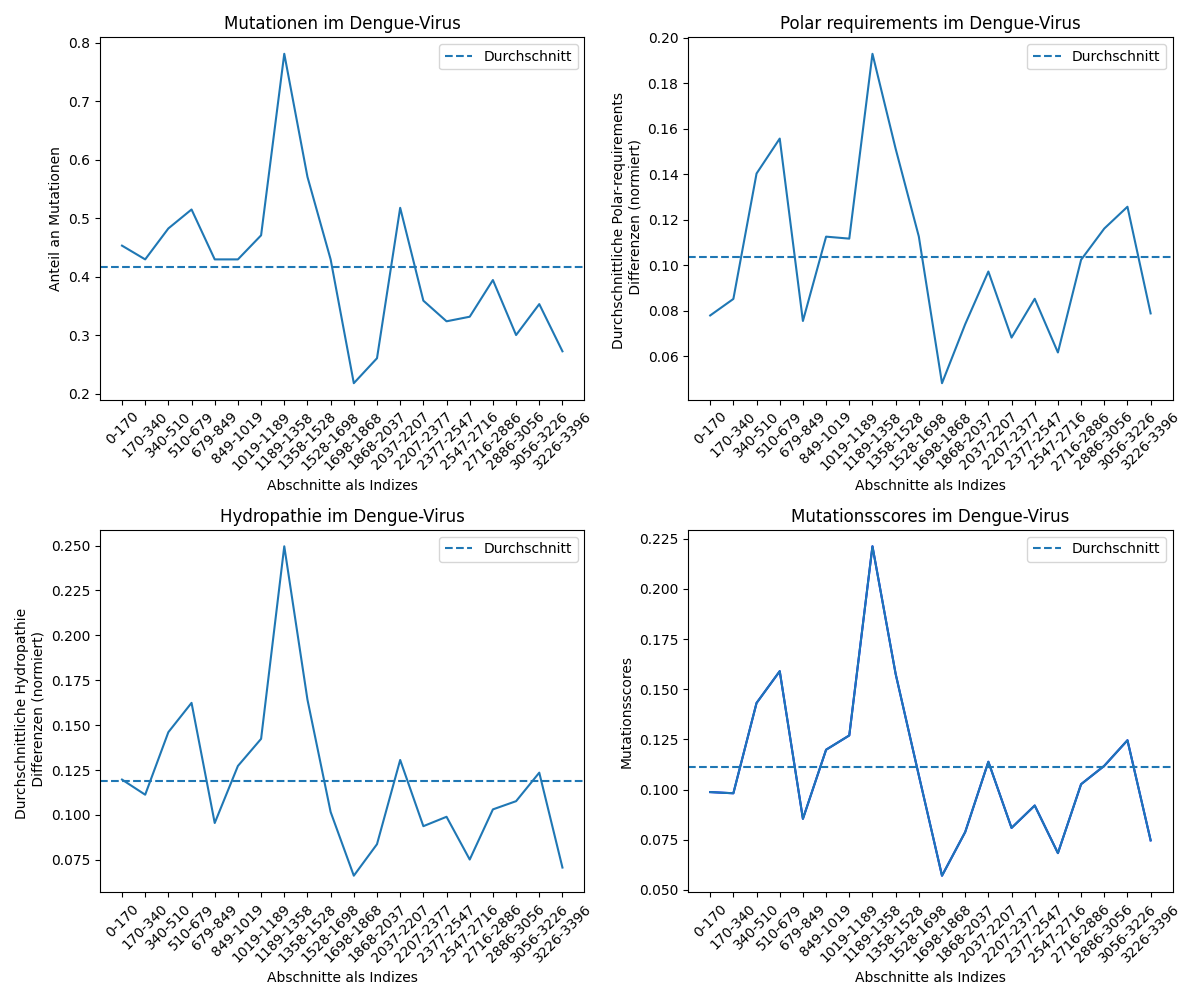
\includegraphics[scale=0.36]{Images/Diagramm_combined_pictures_Dengue_virus.png}
  \caption{Darstellung der Analyseergebnisse f\"ur das Dengue-Virus in vier Subplots: Oben links: Anteil an Mutationen im Polyprotein des Dengue-Virus, wobei das Maximum bei 0,78 in dem Abschnitt 1189-1358 und das Minimum bei 0,22 in 1698-1868 liegt. Oben rechts: Durchschnittliche normierte Polar-Requirement-Differenzen, mit einem Maximum von 0,19 in 1189-1358 und einem Minimum von 0,05 in 1698-1868. Unten links: Durchschnittliche normierte Hydropathie-Differenzen, die ein Maximum von 0,25 in 1189-1358 und ein Minimum von 0,07 in 1698-1868 zeigen. Unten rechts: Mutationsscore \"uber die 20 Teilsequenzen des Dengue-Virus, mit einem Maximum von 0,22 in 1189-1358 und einem Minimum von 0,06 in 1698-1868. Die x-Achse in allen Subplots zeigt die 20 Aminos\"aureabschnitte des Dengue-Virus mit Indizes von 0-170 bis 3226-3396. Diese Abbildung veranschaulicht die Variabilit\"at der Mutationen und deren Auswirkungen auf die Polar-Requirement und Hydropathie im Dengue-Virus.}
  \label{fig:Dengue_virus_combined}
\end{figure}


Im ersten Berechnungsschritt wurde der Anteil an Mutationen vom Polyprotein des Dengue-Virus berechnet. Die Ergebnisse sieht man in der Abbildung \ref{fig:Dengue_virus_combined} oben links. Auf der x-Achse sind die 20 Aminos\"aureabschnitte des Dengue-Virus mit Indexen aufgelistet, von 0-170 bis 3226-3396. Die y-Achse zeigt den Anteil an Mutationen an. Das Maximum wird in dem Abschnitt 1189-1358 erreicht und betr\"agt 0,78, w\"ahrend das Minimum bei 1698-1868 liegt und 0,22 betr\"agt. Die Spannweite der Werte liegt somit bei 0,56. Der Durchschnittswert der Datenpunkte liegt bei 0,42. 

Anschlie\ss{}end wurden die durchschnittlichen normierten Polar-Requirement-Differenzen f\"ur eine Teilsequenz berechnet. Die Ergebnisse sind in der Abbildung \ref{fig:Dengue_virus_combined} oben rechts aufgezeichnet. Auf der x-Achse sind die 20 Aminos\"aureabschnitte des Dengue-Virus mit Indexen aufgelistet, von 0-170 bis 3226-3396. Die y-Achse zeigt die durchschnittlichen normierten Polar-Requirement-Differenzen an. Das Maximum wird in dem Abschnitt 1189-1358 erreicht und betr\"agt 0,19, w\"ahrend das Minimum bei 1698-1868 liegt und 0,05 betr\"agt. Die Spannweite der Werte liegt somit bei 0,14. Der Durchschnittswert der Datenpunkte liegt bei 0,10. 

Auch f\"ur die Hydropathie Werte wurden die durchschnittlichen normierten Differenzen f\"ur eine Teilsequenz berechnet. Die Ergebnisse sind in der Abbildung \ref{fig:Dengue_virus_combined} unten links aufgezeichnet. Auf der x-Achse sind die 20 Aminos\"aureabschnitte des Dengue-Virus mit Indexen aufgelistet, von 0-170 bis 3226-3396. Die y-Achse zeigt die durchschnittlichen normierten Hydropathie Differenzen an. Das Maximum wird in dem Abschnitt 1189-1358 erreicht und betr\"agt 0,25, w\"ahrend das Minimum bei 1698-1868 liegt und 0,07 betr\"agt. Die Spannweite der Werte liegt somit bei 0,18. Der Durchschnittswert der Datenpunkte liegt bei 0,12.

Die Ergebnisse von der Berechnung des Mutationsscores \"uber die 20 Teilsequenzen des Dengue-Virus sind in der Abbildung \ref{fig:Dengue_virus_combined} unten rechts zu finden. Auf der x-Achse sind die 20 Aminos\"aureabschnitte des Dengue-Virus mit Indexen aufgelistet, von 0-170 bis 3226-3396. Die y-Achse zeigt den Mutationsscore an. Das Maximum wird in dem Abschnitt 1189-1358 erreicht und betr\"agt 0,22, w\"ahrend das Minimum bei 1698-1868 liegt und 0,06 betr\"agt. Die Spannweite der Werte liegt somit bei 0,16. Der Durchschnittswert der Datenpunkte liegt bei 0,11. 

Abbildung \ref{fig:Dengue_virus_scores_and_mutations_bereiche} kombiniert den Mutationsscore und den Anteil an Mutationen in einem Diagramm. Auf der x-Achse sind die 20 Aminos\"aureabschnitte des Dengue-Virus mit Indexen aufgelistet, von 0-170 bis 3226-3396. Es gibt zwei y-Achsen. Auf der linken (roten) y-Achse wird der Mutationsscore angezeigt. Auf der rechten (blauen) y-Achse wird der Anteil an Mutationen angezeigt. Die Daten sind entsprechend gef\"arbt. Die Werte entsprechen somit den vorangegangenen Ergebnissen in Abbildung \ref{fig:Dengue_virus_combined}. Au\ss{}erdem befinden sich Maxima und Minima an denselben Stellen. Weiterhin erkennt man, dass die beiden Linien sich \"ahneln und der Durchschnitt jeweils an einer \"ahnlichen Stelle liegt im Vergleich zum jeweiligen Wertebereich. An wenigen Stellen liegen die errechneten Werte weit auseinander, zum Beispiel bei 0-170, 679-849 und 3056-3226.
\begin{figure}[tbp]
  \centering
  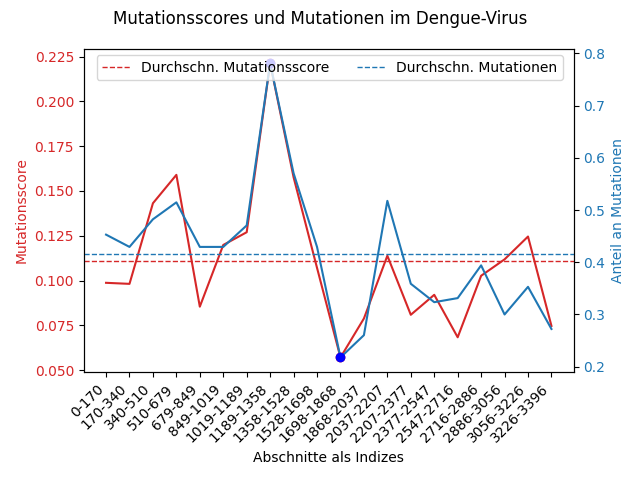
\includegraphics[scale=0.65]{Images/Diagramm_Scores_und_Mutationen_Dengue_viren_Bereiche.png}
  \caption{Diagramm zur Analyse der Mutationen und Scores im Dengue-Virus, das die automatische Aufteilung der Sequenzen in 20 gleich gro\ss{}e Bereiche zeigt. Auf der x-Achse sind die 20 Aminos\"aureabschnitte des Dengue-Virus mit Indizes von 0-170 bis 3226-3396 aufgelistet. Die linke (rote) y-Achse zeigt den Mutationsscore an, w\"ahrend die rechte (blaue) y-Achse den Anteil an Mutationen darstellt. Die Daten verdeutlichen, dass Maxima und Minima in denselben Abschnitten auftreten und die beiden Linien sich \"ahnlich verhalten, was auf eine signifikante Korrelation zwischen den analysierten Parametern hinweist.}
  \label{fig:Dengue_virus_scores_and_mutations_bereiche}
\end{figure}

In der Abbildung \ref{fig:Dengue_virus_scores_and_mutations_bereiche_random} sind die Ergebnisse von der Berechnung des Mutationsscores und dem Anteil an Mutationen f\"ur die zuf\"allige Permutation des Polyproteins zu sehen. Auf der x-Achse sind die 20 Aminos\"aureabschnitte des Dengue-Virus mit Indexen aufgelistet, von 0-170 bis 3226-3396. Es gibt zwei y-Achsen. Auf der linken (roten) y-Achse wird der Mutationsscore angezeigt. Auf der rechten (blauen) y-Achse wird der Anteil an Mutationen angezeigt. Die Daten sind entsprechend gef\"arbt. Das Maximum des Mutationsscores wird in dem Abschnitt 2207-2377 erreicht und betr\"agt 0,14, w\"ahrend das Minimum bei 1698-1868 liegt und 0,08 betr\"agt. Die Spannweite der Werte liegt somit bei 0,06. Der Durchschnittswert der Datenpunkte liegt bei 0,11. Das Maximum des Anteils an Mutationen wird in dem Abschnitt 679-849 erreicht und betr\"agt 0,46, w\"ahrend das Minimum bei 1698-1868 liegt und 0,36 betr\"agt. Die Spannweite der Werte liegt somit bei 0,10. Der Durchschnittswert der Datenpunkte liegt bei 0,42.
\begin{figure}[tbp]
  \centering
  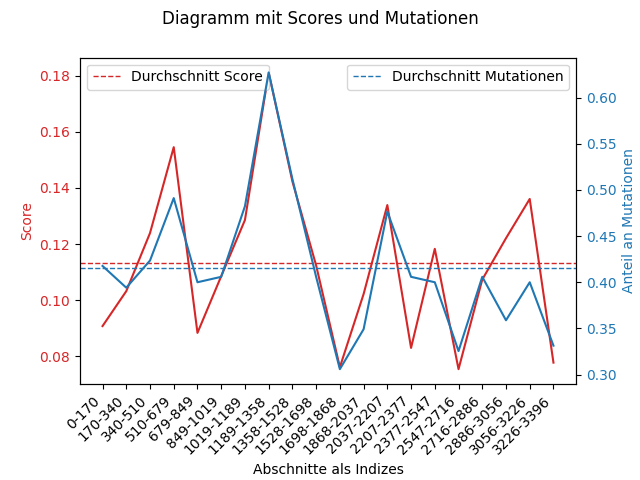
\includegraphics[scale=0.65]{Images/Diagramm_Scores_und_Mutationen_Dengue_viren_Bereiche_random.png}
  \caption{Diagramm zur Analyse der Scores und Mutationen im Dengue-Virus, das die automatische Aufteilung der Sequenzen in 20 gleich gro\ss{}e Bereiche mit einer zuf\"alligen Permutation des Dengue-Virus zeigt. Die Permutation wurde durch 10.000 Vertauschungen durchgef\"uhrt. Auf der x-Achse sind die 20 Aminos\"aureabschnitte des Dengue-Virus mit Indizes von 0-170 bis 3226-3396 aufgelistet. Die linke (rote) y-Achse zeigt den Mutationsscore an, w\"ahrend die rechte (blaue) y-Achse den Anteil an Mutationen darstellt.}
  \label{fig:Dengue_virus_scores_and_mutations_bereiche_random}
\end{figure}

Die Ergebnisse f\"ur die Berechnung des Mutationsscores und des Anteils an Mutationen auf Grundlage der einzelnen Proteine des Dengue-Virus sind in der Abbildung \ref{fig:Dengue_virus_scores_and_mutations_namen} zu sehen. Auf der x-Achse sind die 13 Proteine des Dengue-Virus aufgelistet. Es gibt zwei y-Achsen. Auf der linken (roten) y-Achse wird der Mutationsscore angezeigt. Auf der rechten (blauen) y-Achse wird der Anteil an Mutationen angezeigt. Die Daten sind entsprechend gef\"arbt. Das Maximum des Mutationsscores wird beim Protein NS2A erreicht und betr\"agt 0,22, w\"ahrend das Minimum bei NS4B liegt und 0,07 betr\"agt. Die Spannweite der Werte liegt somit bei 0,15. Der Durchschnittswert der Datenpunkte liegt bei 0,12. Das Maximum des Anteils an Mutationen wird beim Protein NS2A erreicht und betr\"agt 0,81, w\"ahrend das Minimum beim Protein NS4B liegt und 0,31 betr\"agt. Die Spannweite der Werte liegt somit bei 0,50. Der Durchschnittswert der Datenpunkte liegt bei 0,48. Neben den Proteinen NS2A und NS4B hat auch das Protein NS3 vergleichsweise extreme Werte. Sowohl beim Anteil an Mutationen als auch beim Mutationsscore liegen die Werte weit unter dem Durchschnitt und sind \"ahnlich extrem wie bei NS4B. Alle anderen Proteine sind in der N\"ahe des Durchschnitts und zeigen keine so extremen Werte, wie NS2A, NS3 und NS4B. 
\begin{figure}[tbp]
  \centering
  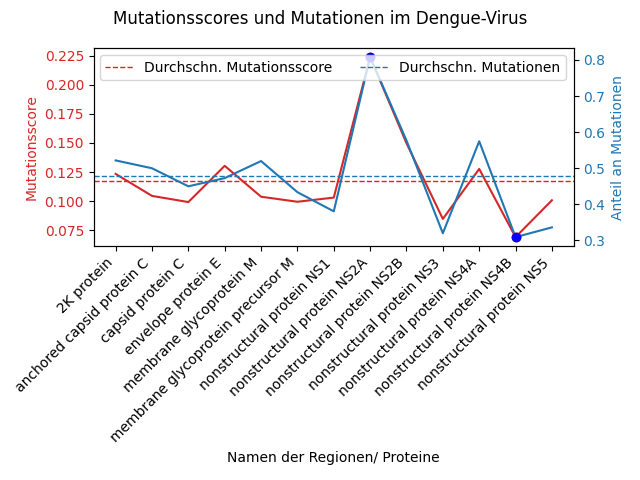
\includegraphics[scale=0.65]{Images/Diagramm_Scores_und_Mutationen_Dengue_viren_Namen.png}
  \caption{Diagramm zur Analyse des Mutationsscores und des Anteils an Mutationen f\"ur die einzelnen Proteine des Dengue-Virus. Auf der x-Achse sind die 13 Proteine mit ihren jeweiligen Bezeichnungen aufgelistet. Die linke (rote) y-Achse zeigt den Mutationsscore an, w\"ahrend die rechte (blaue) y-Achse den Anteil an Mutationen darstellt. Das Maximum des Mutationsscores wird beim Protein NS2A erreicht (0,22), w\"ahrend das Minimum bei NS4B liegt (0,07). Der Anteil an Mutationen erreicht ebenfalls sein Maximum bei NS2A (0,81) und sein Minimum bei NS4B (0,31).}
  \label{fig:Dengue_virus_scores_and_mutations_namen}
\end{figure}


\chapter{Diskussion}
In diesem Kapitel werden die Ergebnisse der vorhergehenden Analysen diskutiert und in den Kontext bestehender wissenschaftlicher Erkenntnisse eingeordnet. Die Analyse der Mutationsstabilit\"at von Transmembranproteinen des Dengue-Virus bietet wertvolle Einblicke in die evolution\"aren Dynamiken und strukturellen Anforderungen dieser Proteine. Besonderes Augenmerk liegt auf den signifikanten Unterschieden in den Mutationsraten der verschiedenen Proteine, insbesondere zwischen den Transmembranproteinen NS2A, NS3 und NS4B. Diese Unterschiede werfen wichtige Fragen zur Funktionalit\"at und zum evolution\"aren Druck auf, dem diese Proteine ausgesetzt sind. In den folgenden Abschnitten werden die spezifischen Ergebnisse detailliert er\"ortert, um ein besseres Verst\"andnis f\"ur die biologischen Implikationen dieser Mutationsmuster zu gewinnen und m\"ogliche zuk\"unftige Forschungsrichtungen aufzuzeigen.

\section{Ergebnisse}
In der Abbildung \ref{fig:Dengue_virus_scores_and_mutations_bereiche} sind starke Abweichungen von den durchschnittlichen Werten f\"ur den Score und den Anteil an Mutationen zu erkennen. Insbesondere bei den Abschnitten 1189-1358 und 1698-1868 ist ein Maximum beziehungsweise ein Minimum zu beobachten. Um zu sch\"atzen, ob diese Extrema signifikant sind und nicht nur zuf\"alligen Schwankungen unterliegen, betrachten wir die Abbildung \ref{fig:Dengue_virus_scores_and_mutations_bereiche_random}, in der die Sequenz zuf\"allig permutiert wurde. Wenn die Extrema zuf\"allige Schwankungen sind, k\"onnen wir annehmen, dass, wenn wir die Sequenz zuf\"allig stellenweise vertauschen, dass dann Extrema weiterhin im selben Ausma\ss{} vorkommen. Wenn die Extrema nicht auf Zufall basieren, sollten die Extrema in der zuf\"allig permutierten Sequenz abgeschw\"acht auftreten; die Werte sollten sich also dem Durchschnitt ann\"ahern. Die starken H\"aufungen von Mutationen oder die starken regionalen Ver\"anderungen im Score wurden abgeschw\"acht, indem einzelne Stellen aus diesem Bereich mit Stellen aus anderen Bereichen der Sequenz, in denen weniger Mutationen oder gro\ss{}e Differenzen im Score zu finden sind, vertauscht wurden. Da die Vertauschungen jedoch zuf\"allig ausgef\"uhrt wurden, existiert kein Bias dar\"uber, welche Stellen ausgew\"ahlt und vertauscht wurden. Sollten die Extrema also zuf\"allig entstanden sein, sollten sich nun an einigen Stellen in der Sequenz wieder geh\"auft Mutationen finden lassen oder starke Ver\"anderungen im Score bestehen. 
In Abbildung \ref{fig:Dengue_virus_scores_and_mutations_bereiche_random} ist erkennbar, dass der Bereich, \"uber den sich die Werte erstrecken, verkleinert ist, im Vergleich zur Abbildung \ref{fig:Dengue_virus_scores_and_mutations_bereiche}. Die Abbildung \ref{fig:Dengue_virus_scores_and_mutations_bereiche_random} hat einen Wertebereich mit einer Spannweite von 0,06 f\"ur den Mutationsscore und einen Wertebereich mit einer Spannweite von 0,1 bei dem Anteil des Mutationsscores. Die Abbildung \ref{fig:Dengue_virus_scores_and_mutations_bereiche} hat einen Wertebereich mit einer Spannweite von 0,16 f\"ur den Mutationsscore und ist damit deutlich gr\"o\ss{}er als bei der zuf\"alligen Permutation. Der Wertebereich f\"ur den Anteil an Mutationen hat eine Spannweite von 0,56. Auch hier ist die Spannweite des Wertebereiches deutlich vergr\"o\ss{}ert im Vergleich zur zuf\"alligen Permutation. Au\ss{}erdem ist klar erkennbar, dass die Extrema stark abgeschw\"acht sind, wodurch anzunehmen ist, dass die Extrema nicht nur zuf\"allig entstanden sind. Daher nehmen wir an, dass die Ergebnisse auch signifikant sind, da die Werte nicht nur zuf\"alligen Schwankungen unterliegen.  

Um die Fragestellung zu beantworten, betrachten wir die Abbildung \ref{fig:Dengue_virus_scores_and_mutations_namen}. Hierbei f\"allt direkt auf, dass die Proteine NS2A, NS3 und NS4B besonders extreme Werte aufweisen, sowohl bei dem Mutationsscore als auch bei dem Anteil an Mutationen. Das Protein NS2A hat dabei besonders hohe Werte, weshalb davon auszugehen ist, dass kein besonders starker Konservierungsdruck in diesem Protein vorhanden sein kann, sondern das Protein eher einem gro\ss{}en Mutationsdruck unterliegt und besonders h\"aufig mutiert. Die Proteine NS3 und NS4B weisen hingegen besonders niedrige Werte auf, sodass von einem starken Konservierungsdruck und einem sehr niedrigen Mutationsdruck innerhalb der Proteine ausgegangen werden kann. 

Die Analyse der Mutationsraten von den Proteinen NS2A, NS3 und NS4B des Dengue-Virus zeigt signifikante Unterschiede in der Konservierung der Proteine. W\"ahrend NS3 und NS4B, die beide Transmembrandom\"anen aufweisen, sich in \"Ubereinstimmung mit den Erwartungen als stark konserviert herausstellen, zeigt NS2A eine unerwartet hohe Mutationsrate. Diese Beobachtung wirft Fragen zur evolution\"aren Dynamik und zur funktionalen Rolle von NS2A auf. Transmembranproteine m\"ussen stark konserviert sein, da ihre Struktur und Funktion eng mit den hydrophoben Anforderungen und den Polar-Requirement ihrer Umgebung verbunden sind. In diesem Kontext ist es nicht \"uberraschend, dass NS3 und NS4B, die beide in die Membran integriert sind, eine hohe Konservierung aufweisen; diese Proteine sind entscheidend f\"ur die virale Replikation und Interaktion mit zellul\"aren Komponenten, was ihre strukturelle Integrit\"at und Funktionalit\"at erfordert. Im Gegensatz dazu k\"onnte die hohe Mutationsrate von NS2A durch seine spezifische Funktion erkl\"art werden: Dieses Protein spielt eine entscheidende Rolle bei der Virusbildung sowie bei der Modulation der Immunantwort des Wirts. Es befindet sich daher gr\"o\ss{}tenteils an der Au\ss{}enseite der infizierten Zelle und muss daf\"ur die Zellwand durchdringen. Diese Positionierung setzt das Protein direkt dem Immunsystem aus; um einer Erkennung durch die Immunabwehr zu entgehen, k\"onnte das Virus gezwungen sein, NS2A regelm\"a\ss{}ig zu mutieren. Diese Mutation erm\"oglicht es dem Virus, seine antigenen Eigenschaften zu variieren und somit dem Immunsystem zu entkommen. Diese evolution\"are Anpassung erh\"oht die \"Uberlebensf\"ahigkeit des Virus in einem dynamischen immunologischen Umfeld.
Zusammenfassend l\"asst sich sagen, dass die hohe Mutationsrate von NS2A nicht allein durch seine strukturellen Eigenschaften erkl\"art werden kann. Vielmehr stellt sie eine evolution\"are Anpassung dar, um die \"Uberlebensf\"ahigkeit des Virus in einem dynamischen immunologischen Umfeld zu sichern. Dennoch bleibt unklar, ob auch die Transmembrandom\"anen von NS2A stark mutieren oder ob die Mutationen haupts\"achlich in anderen Regionen auftreten. Um daf\"ur eine abschlie\ss{}ende Antwort zu finden, sollte dieses Protein genauer untersucht und die Mutationsraten in den einzelnen Dom\"anen aufgeschl\"usselt werden. 

Die vorliegenden Ergebnisse geben keine eindeutige Antwort darauf, ob Transmembranproteine aufgrund ihrer strukturellen Anforderungen an Polar-Requirement und Hydropathie generell stark konserviert sind. Die unerwartet hohe Mutationsrate von NS2A deutet darauf hin, dass auch Transmembranproteine unter bestimmten funktionellen Zw\"angen stehen k\"onnen, die zu einer erh\"ohten Mutationsrate f\"uhren. Eine detaillierte Analyse der Mutationsmuster in den einzelnen Dom\"anen der untersuchten Proteine k\"onnte wertvolle Einblicke in die Faktoren liefern, die die Konservierung von Transmembranproteinen beeinflussen.

\section{Datens\"atze erweitern}
Um die Aussagekraft der Ergebnisse zur Mutationsrate von Dengue-Virus-Proteinen zu verbessern, muss die Datengrundlage erweitert werden. Es gibt zwei Ans\"atze, die das Programm weiterentwickeln k\"onnen. Entweder man untersucht die Proteine detaillierter auf Dom\"anenebene, um herauszufinden, ob einzelne Proteine trotz hohem Mutationsdruck in bestimmten Dom\"anen besonders konserviert sind. Oder man erweitert den Datensatz auf mehr verschiedene Viren oder sogar andere DNA-Str\"ange, um die Verallgemeinerbarkeit der Beobachtungen zu \"uberpr\"ufen. Die folgenden Abschnitte werden n\"aher auf die Umsetzung und Implikationen dieser beiden Ans\"atze eingehen.

\subsection{Untersuchung von Dom\"anen}
Die gegenw\"artige Analyse konzentriert sich auf die Serotypen des Dengue-Virus und untersucht spezifisch die einzelnen Proteine, ohne dabei die zugrunde liegenden Dom\"anen zu ber\"ucksichtigen. Diese Fokussierung bietet wertvolle Einblicke in die Mutationsdynamik der Proteine, jedoch nicht in die Mutationsdynamik der Dom\"anen. Ein m\"oglicher Ansatz zur Untersuchung, ob einzelne Proteine trotz ihres generell hohen Mutationsdrucks in den Transmembrandom\"anen besonders stark konserviert sind, ist den bestehenden Code so anzupassen, dass er die Analyse der Transmembrandom\"anen erm\"oglicht und nicht nur ganze Proteine als Berechnungsgrundlage erh\"alt. Dies w\"urde ein detaillierteres Verst\"andnis ihrer konservativen Eigenschaften in Bezug auf Polar-Requirement und Hydropathie bieten. Um dies umzusetzen, m\"usste man manuell annotiert einen Ordner f\"ur jedes Protein erstellen. Jede Dom\"ane w\"urde dann in einer eigenen FASTA-Datei gespeichert, wobei der entsprechende DNA-Abschnitt jedes Serotyps in der Datei enthalten ist. Diese einzelnen FASTA-Dateien m\"ussten anschlie\ss{}end ausgerichtet werden. Der gesamte Ordner k\"onnte dann eingelesen und berechnet werden, ohne dass das Programm weiter angepasst werden muss. Da das Erstellen dieser Dateien jedoch einen erheblichen Aufwand erfordert, k\"onnte das vorhandene Programm auch verwendet werden, um Ordner automatisch zu generieren. Aktuell kann das Programm nur f\"ur das gesamte Polyprotein Ordner erstellen, in denen die einzelnen Proteine gespeichert sind (siehe Kapitel Materialien und Methoden). Eine Anpassung des Programms w\"urde es erm\"oglichen, auch die einzelnen Dom\"anen aus annotierten GenBank-Daten auszulesen und somit eine neue Ordnerstruktur halb automatisch zu erstellen. Obwohl das Anpassen des Programms m\"oglich ist, bleibt es notwendig, die einzelnen Dom\"anen aus den Proteinen manuell mit den entsprechenden Dom\"anen anderer Serotypen abzugleichen und in einer Datei zusammenzuf\"uhren. Auch diese Dateien m\"ussen anschlie\ss{}end ausgerichtet werden. Daher kann zwar der Arbeitsaufwand reduziert werden, dennoch bleibt ein gewisser zeitlicher Aufwand bestehen. Bei Bedarf sollte daher der bestehende Code erweitert werden, um die geforderte Ordnerstruktur automatisch zu generieren.

\subsection{Automatische Eingaben}
Wie im vorangegangenen Abschnitt erw\"ahnt, wird manuelle Arbeit ben\"otigt, um Eingaben f\"ur das genutzte Programm zu erstellen. Dieser Aufwand kann erheblich sein und wird insbesondere dann hinderlich, wenn das Programm mit neuen Daten erweitert werden soll. Bei gro\ss{}en Datenmengen wird der Zeitaufwand so gro\ss{}, dass die manuelle Erstellung der Eingaben nicht mehr realistisch ist. Daher sollte das Programm f\"ur gr\"o\ss{}ere Datens\"atze erweitert werden, um Eingaben automatisch zu generieren und zu erm\"oglichen, dass die Datengrundlage auf weitere Viren und andere DNA-Str\"ange ausgeweitet werden kann. Aktuell kann zwar automatisch ein Ordner f\"ur einen Serotypen erstellt werden, der alle Proteine des Dengue-Virus enth\"alt, sofern diese in GenBank annotiert sind. Im n\"achsten Schritt m\"ussen jedoch f\"ur jedes gefundene Protein die entsprechenden Dateien aus verschiedenen Serotypen gesucht und zusammengef\"uhrt werden, um sie anschlie\ss{}end auszurichten und als Eingabe zu verwenden. Dieser Prozess muss bei gro\ss{}en Datenmengen automatisiert erfolgen, um in einem sinnvollen Zeitrahmen zu bleiben. Die Automatisierung dieses Schrittes gestaltet sich jedoch als komplex, da die Daten aus GenBank nicht vollst\"andig standardisiert sind. Das Auffinden der entsprechenden Proteine wird dadurch erschwert. Beispielsweise wird das 2K-Peptid im Dengue-Virus in einer Studie als "`protein 2K"' benannt und in einer anderen als "`2K protein"'. Die Dateinamen variieren also erheblich. Der Algorithmus muss daher so trainiert werden, dass er mit diesen unterschiedlichen Bezeichnungen umgehen kann und dennoch die korrekten Dateien findet. Diese Algorithmen werden als Matching-Algorithmen bezeichnet und sind Gegenstand aktueller Forschung~\cite{jurafsky2020speech, manning2008introduction, zhang2019survey}. Dieses Problem tritt auch auf, wenn man die Ordnerstruktur vollautomatisch f\"ur Dom\"anen anstelle von Proteinen erstellen m\"ochte, wie im vorherigen Abschnitt besprochen.

\subsection{Untersuchung weiterer Viren und DNA-Str\"ange}
Um die Fragestellung abschlie\ss{}end zu kl\"aren, muss der Datensatz auf weitere DNA-Str\"ange ausgeweitet werden. Nur eine umfassendere Datengrundlage w\"urde es erm\"oglichen, festzustellen, ob die beobachteten Muster spezifisch f\"ur das Dengue-Virus sind oder auch auf andere Viren zutreffen. Es ist jedoch wichtig zu beachten, dass der Vergleich verschiedener Viren in kleinen Datens\"atzen nicht zielf\"uhrend ist. Die Literatur unterst\"utzt die Auffassung, dass eine eingehende Analyse des Mutationsmusters eines einzelnen Virus sinnvoller ist, um pr\"azise Ergebnisse f\"ur einzelne Proteine zu erzielen~\cite{nina}. In dieser Arbeit werden jedoch Transmembrandom\"anen unabh\"angig von spezifischen, einzelnen Proteinen untersucht. Es wird versucht, eine allgemeing\"ultige Aussage \"uber die Konservierung von Transmembranproteinen zu treffen. Daf\"ur ist es notwendig, \"uber das Dengue-Virus hinauszugehen und weitere Viren zu untersuchen. Das Programm erlaubt bereits die Eingabe verschiedenster DNA-Datens\"atze und ist nicht auf das Dengue-Virus beschr\"ankt. Es ist m\"oglich, die Eingaben gegen andere DNA-Sequenzen auszutauschen oder den Code so zu erweitern, dass mehr Eingaben eingelesen und berechnet werden k\"onnen. Allerdings erfordert dies einen gr\"o\ss{}eren Aufwand, da f\"ur die Berechnung der Werte f\"ur einzelne Proteine ein Ordner mit FASTA-Dateien erstellt werden muss. Im Kapitel Materialien und Methoden wird n\"aher darauf eingegangen. Das manuelle Zusammenkopieren und Ausrichten dieser Dateien ist bei kleinen Datens\"atzen m\"oglich, wird jedoch schnell sehr zeitaufw\"andig. Je mehr Proteine untersucht werden sollen, desto h\"oher wird der Zeitaufwand, insbesondere wenn es mehr Serotypen pro Virus gibt. Daher wird es notwendig sein, das Programm zu erweitern und das Einlesen von Dateien zu vereinfachen. Die Umsetzung dessen wurde bereits ausf\"uhrlich im vorherigen Teil diskutiert. Dar\"uber hinaus kann auch das Ausrichten der Datens\"atze automatisiert werden. Nach dem Matching-Prozess k\"onnten die Proteine automatisch in einen Ausrichtungsalgorithmus gegeben werden, wobei die Ausgabe direkt in die Berechnung eingeht. Da ein automatischer Matching-Prozess jedoch sehr komplex ist, k\"onnte man auch darauf verzichten, die DNA-Str\"ange in spezifische Bereiche wie Proteine zu unterteilen und stattdessen den DNA-Strang in gleich gro\ss{}e Abschnitte aufzuteilen. Dieser Ansatz wurde bereits in dieser Arbeit bei Abbildung \ref{fig:Dengue_virus_scores_and_mutations_bereiche} angewendet und im Kapitel Materialien und Methoden beschrieben. Dieser Ansatz ist deutlich einfacher auf gro\ss{}e Datens\"atze anzuwenden, weil f\"ur ein Virus mit vielen Serotypen und Proteinen nur eine Datei erstellt und ausgerichtet werden muss. Es ist keine weitere Arbeit im Vorfeld n\"otig. Die Unterteilung in Abschnitte funktioniert vollautomatisiert und kann angepasst werden, indem die Anzahl der Sequenzteile eingegeben wird. So kann individuell entschieden werden, in wie viele Teile die Sequenzen unterteilt werden sollen und damit wie granular die Berechnung ist. Diese Methode eignet sich auch f\"ur Datens\"atze, \"uber die man nur wenig Kenntnis hat. Beispielsweise kann man auch ein Polyprotein, dessen genaue Proteinpositionen unbekannt sind, untersuchen und kann diese Berechnung dennoch durchf\"uhren, da nicht auf die einzelnen Proteingrenzen geachtet werden muss. Somit kann man auch f\"ur diese Datens\"atze eine Aussage \"uber die Mutationsdynamik treffen.  

Dar\"uber hinaus wurde das aktuelle Programm in Python entwickelt. W\"ahrend dies f\"ur kleinere Datens\"atze praktikabel ist, st\"o\ss{}t es bei gr\"o\ss{}eren Datenmengen und komplexeren Analysen an seine Leistungsgrenzen. Python ist nicht auf Performanz optimiert; gro\ss{}e Datenmengen k\"onnen dazu f\"uhren, dass Berechnungen nicht mehr in einem sinnvollen Zeitrahmen abgeschlossen werden k\"onnen. Auch T-Coffee, das genutzte Ausrichtungswerkzeug, ist nicht f\"ur gro\ss{}e Datenmengen optimiert. Es ist ein sehr pr\"azises Ausrichtungswerkzeug und deshalb geeignet, kurze DNA-Str\"ange sinnvoll auszurichten. Bei gro\ss{}en Datenmengen und langen DNA-Str\"angen kann es sinnvoll sein, schnellere und weniger pr\"azise Ausrichtungswerkzeuge zu verwenden. In solchen F\"allen fallen einzelne Fehler in gro\ss{}en Datens\"atzen nicht so stark ins Gewicht, sodass eine geringere Pr\"azision dennoch ausreichend sein kann.

\section{Berechnungsgrundlagen}
Neben der Erweiterung der Datens\"atze k\"onnen auch die Berechnungsgrundlagen angepasst werden. Im aktuellen Programm werden bei der Berechnung des Anteils an Mutationen L\"ucken ber\"ucksichtigt. Bei der Berechnung des Scores hingegen nicht. L\"ucken entstehen h\"aufig in biologischen Sequenzen, wenn Mutationen auftreten. Sie sind wichtig, um die Struktur und Evolution von Sequenzen korrekt darzustellen. Ihre Ber\"ucksichtigung bei der Berechnung des Mutationsanteils ist sinnvoll, da sie die tats\"achliche Variation in der Sequenz widerspiegeln. Der Score hingegen basiert auf den Werten f\"ur Polar-Requirement und Hydropathie. Da L\"ucken keine Werte in Bezug auf diese Eigenschaften haben, werden sie bei der Score-Berechnung nicht ber\"ucksichtigt. Wenn eine L\"ucke als Mutation gez\"ahlt wird, aber nicht im Score reflektiert wird, k\"onnte dies zu einer irref\"uhrenden Interpretation der biologischen Bedeutung f\"uhren. Ein hoher Anteil an Mutationen k\"onnte f\"alschlicherweise als biologisch relevant angesehen werden, w\"ahrend der Score nicht entsprechend angepasst ist. Die Diskrepanz k\"onnte dazu f\"uhren, dass bestimmte Sequenzen irrt\"umlich als weniger oder mehr stabil angesehen werden, was Auswirkungen auf nachfolgende Analysen oder Anwendungen haben k\"onnte. Deshalb wurden in dieser Arbeit immer beide Werte, Mutationsanteil und Score, angegeben (siehe Abbildung \ref{fig:Dengue_virus_scores_and_mutations_namen}). Weiterhin w\"are es sinnvoll zu \"uberlegen, wie L\"ucken sowohl in der Mutationsberechnung als auch im Score ber\"ucksichtigt werden k\"onnen. Eine m\"ogliche L\"osung k\"onnte sein, L\"ucken einen spezifischen Wert oder Einfluss auf den Score zuzuweisen. Beispielsweise k\"onnte man einer L\"ucke den Mittelwert \"uber die Polar-Requirement zuweisen, um einen Standardwert zu haben. Allerdings f\"uhrt dies zu einer Verzerrung des Scores. Beispielsweise k\"onnte dadurch in Bereichen, in denen die Polar-Requirement-Werte konstant sehr hoch sind, der Score diese Tatsache nicht korrekt widerspiegeln. Der Score gibt bisher immer starke \"Anderungen innerhalb von Polar-Requirement oder Hydropathie an, wenn sich die Werte zwischen den Serotypen stark unterscheiden, dann wird der Score gr\"o\ss{}er. Tritt nun in einer Sequenz mit ansonsten konstant hohen Werten eine L\"ucke auf, wird der Score automatisch erh\"oht, da der L\"ucken-Wert deutlich niedriger liegt als die Werte der anderen Serotype. Dadurch wird der Score verf\"alscht.

Dar\"uber hinaus kann man die grunds\"atzliche Berechnung des Scores hinterfragen. F\"ur die Score-Berechnung wird der Durchschnitt \"uber die normierten Differenzen von Polar-Requirement und Hydropathie gemittelt. Der Durchschnitt ist jedoch nicht immer ein geeignetes Mittel, da er sehr empfindlich auf Ausrei\ss{}er reagiert. Fehler in der Datenerhebung k\"onnten das Ergebnis stark verzerren. Da wir aber gerade nach solchen Extremwerten suchen, die auf wichtige Funktions\"anderungen hinweisen und uns explizit f\"ur diese "`Ausrei\ss{}er"' interessieren, ist der Durchschnitt besser geeignet als beispielsweise die Berechnung eines Medians. Wenn ein Protein bereits an wenigen Stellen die biochemischen Grundlagen durch Mutationen stark ver\"andert, kann dies weitreichende Folgen f\"ur die Funktionalit\"at des Virus haben und sogar dessen \"Uberlebensf\"ahigkeit gef\"ahrden. Diese starken Ausrei\ss{}er zu minimieren und im Score zu neutralisieren, widerspricht dem Ziel, gerade diese Mutationen zu identifizieren. Des Weiteren werden die Werte f\"ur die Sequenzteile nicht immer auf gleich gro\ss{}en Sequenzteilen berechnet. Bei der Berechnung der Werte f\"ur die Proteine sind die Sequenzteile nicht mehr gleich lang. Da jedoch beide berechneten Werte anteilig in Bezug auf die L\"ange berechnet werden, bleiben die Werte vergleichbar miteinander.

Au\ss{}erdem ist bei der Berechnung des Scores fragw\"urdig, ob die verwendeten Werte f\"ur Hydropathie und Polar-Requirement korrekt sind. Bei den Hydropathie-Werten wurden vier Werte h\"andisch angepasst, wie bereits im Kapitel Materialien und Methoden erw\"ahnt. Auch bei den Polar-Requirement gab es nachtr\"agliche Anpassungen. Die erhobenen Werte scheinen also Fehlern zu unterliegen. Polar-Requirement wurde in den nachfolgenden Jahren, nach der Ver\"offentlichung der originalen Daten, mehrfach erneut untersucht, zum Beispiel von \citeauthor{mathew_physical_2008}~\cite{mathew_physical_2008}. In der urspr\"unglichen Studie von \citeauthor{woese_fundamental_1966}~\cite{woese_fundamental_1966} lag der Fokus auf der Analyse von RNA-Sequenzen, insbesondere der ribosomalen RNA (rRNA), um phylogenetische Beziehungen zwischen verschiedenen Organismen zu untersuchen. Woese sammelte rRNA-Sequenzen aus verschiedenen Organismen und f\"uhrte einen direkten Vergleich dieser Sequenzen durch. Er verwendete Algorithmen zur Berechnung der \"Ahnlichkeiten und Unterschiede zwischen den Sequenzen, um evolution\"are Verwandtschaften abzuleiten. Auf Basis der gesammelten Sequenzdaten erstellte Woese phylogenetische B\"aume, die die evolution\"aren Beziehungen zwischen den Organismen visualisierten. Diese Methode beruhte stark auf der Annahme, dass genetische Unterschiede auf evolution\"are Divergenz hinweisen. Im Gegensatz dazu verfolgten \citeauthor{mathew_physical_2008}~\cite{mathew_physical_2008} einen experimentellen und physikochemischen Ansatz zur Bestimmung von Polar-Requirement und Hydropathie. \citeauthor{mathew_physical_2008} f\"uhrten pr\"azise experimentelle Messungen durch, um die Polar-Requirement und Hydropathie von Aminos\"auren zu quantifizieren. Diese Werte wurden durch verschiedene biophysikalische Techniken ermittelt, wie z. B. chromatografische Verfahren oder spektroskopische Analysen. In ihrer Studie wurden die urspr\"unglich erhobenen Werte f\"ur Polar-Requirement nachtr\"aglich angepasst, um m\"ogliche Fehler zu korrigieren und genauere Ergebnisse zu gew\"ahrleisten. Dies zeigt eine iterative Herangehensweise, bei der bestehende Daten kritisch hinterfragt und verbessert wurden. \citeauthor{mathew_physical_2008} kombinierten die experimentellen Daten mit theoretischen Modellen, um ein umfassenderes Verst\"andnis der Auswirkungen von Aminos\"aure-Eigenschaften auf die Proteinstruktur zu erreichen. Diese Kombination aus experimenteller und theoretischer Analyse erm\"oglicht eine differenzierte Betrachtung der biologischen Relevanz von Mutationen. Zusammenfassend l\"asst sich sagen, dass die originalen Daten von Woese nicht mehr dem aktuellen Stand der Forschung entsprechen. Es gibt mittlerweile weitere Studien, die versuchen, den validen Polar-Requirement-Werten n\"aherzukommen. In dieser Arbeit wurde jedoch entschieden, die originalen Daten zu verwenden, um vergleichbar mit der vorangegangenen Forschung am Institut~\cite{nina} zu bleiben. Des Weiteren enthalten die Werte von Mathew und Luthey-Schulten keine sehr starken Abweichungen zu den Werten von Woese, weshalb die Abweichungen bei den Grundannahmen aus dieser Arbeit nicht weiter ins Gewicht fallen sollten. Bei weiterer Forschung kann es jedoch sinnvoll sein, die genutzten Werte von Hydropathie und Polar-Requirement weiter zu hinterfragen und gegebenenfalls anzupassen.

\chapter{Fazit}
% In a German thesis write: \subsection{Zusammenfassung und Ausblick}


% !!!!!!!!!!!!!!!!!!!!!!!!!!!!!!!!!!
% !!! Your action is needed here !!!
% !!!!!!!!!!!!!!!!!!!!!!!!!!!!!!!!!!
%
% Replace the following with your conclusion

In dieser Bachelorarbeit wird die Stabilit\"at von Transmembranbereichen innerhalb von Viren in Bezug auf Hydropathie und Polar-Requirement-Werte untersucht, mit einem besonderen Fokus auf das Dengue-Virus. Diese grundlegende Forschung zielt darauf ab, ein besseres Verst\"andnis der biochemischen Eigenschaften von Virusproteinen zu erlangen, die entscheidend f\"ur deren Funktion und Stabilit\"at sind. Hydropathie beschreibt die Affinit\"at von Molek\"ulen zu Wasser, w\"ahrend Polar-Requirement spezifische Anforderungen an die Polarit\"at von Aminos\"auren in Proteinen darstellen. Diese Konzepte klassifizieren Molek\"ule in hydrophile (wasserliebend) und hydrophobe (wasserabweisend) Substanzen und sind besonders wichtig f\"ur die Interaktion von Proteinen mit ihrer Umgebung, insbesondere in biologischen Membranen, wo sich die Polarit\"at der Lipid-Doppelschicht von der des extrazellul\"aren und intrazellul\"aren Raums unterscheidet. In transmembranen Regionen m\"ussen Proteine sowohl hydrophobe als auch hydrophile Bereiche aufweisen, um stabil in der Membran verankert zu sein und ihre Funktion zu erf\"ullen. Mutationen in diesen Schl\"usselbereichen k\"onnen die Stabilit\"at und Funktionalit\"at der Proteine erheblich beeintr\"achtigen, was wiederum Auswirkungen auf die Infektiosit\"at des Virus haben kann. Das Hauptziel dieser Arbeit besteht darin, zu untersuchen, ob transmembrane Dom\"anen im Dengue-Virus hinsichtlich ihrer Hydropathie- und Polar-Requirement-Werte besonders konserviert sind. Diese Untersuchung ist entscheidend f\"ur das Verst\"andnis der Entstehung von Mutationen in diesen Bereichen sowie deren potenziellen Einfluss auf die Stabilit\"at des Virus. Zur Analyse wurden bioinformatische Tools eingesetzt, um Mutationsstabilit\"at innerhalb der Dengue-Viren zu untersuchen. Diese Analyse f\"ordert ein tieferes Verst\"andnis f\"ur die Wechselwirkungen zwischen den transmembranen Bereichen des Dengue-Virus und ihrer Umgebung. Die Ergebnisse zeigen, dass bestimmte Transmembranproteine des Dengue-Virus eine hohe Konservierung aufweisen, was auf einen evolution\"aren Druck hinweist. Diese Erkenntnisse deuten darauf hin, dass diese Viren eine geringere Anf\"alligkeit f\"ur Mutationen aufweisen. Dennoch geben die Ergebnisse keine eindeutige Antwort auf alle Fragen zur Mutationsstabilit\"at; vielmehr zeigen sie die Notwendigkeit weiterer Forschung. Zuk\"unftige Studien sollten sich darauf konzentrieren, spezifische Viren und deren Mutationsmuster in Bezug auf konkrete Dom\"anen eingehender zu untersuchen. Insgesamt bietet diese Bachelorarbeit wertvolle Einblicke in die biochemischen Eigenschaften von Virusproteinen und deren Stabilit\"at in Bezug auf Hydropathie und Polar-Requirement. Die Erkenntnisse tragen dazu bei, ein besseres Verst\"andnis der Mutationsmechanismen zu entwickeln und sind entscheidend f\"ur das Verst\"andnis der Virusbiologie sowie der Erforschung von Mutationsmustern in verschiedenen Arten von DNA-Sequenzen.




% Normally, the bibliography comes next at this point. Do *not* (try
% to) include further indices and tables like an index or
% a list of figures or a list of tables or such things. Nobody
% actually uses them and they just use up space. 
%
% You *can* however include a glossary, if this seems appropriate. It
% goes here as an unnumbered chapter. Most thesis will *not* need a
% glossary: a well-written text (re)explains strange words and
% concepts as necessary. However, there are situations where a
% glossary may be helpful.














%%%
% 
% Bibliographies
%
%%%
%
% The uzl-thesis class will load biblatex for the bibliography
% management. This is a powerful package, see its documentation for
% details. The styles will be setup correctly and automatically by
% choosing one of the two style keys as described earlier.
%
% In order for the bibliography to work, run latex in the following
% order (which is the standard order):
% 
% > lualatex thesis-example
% > bibtex thesis-example
% > lualatex thesis-example
% 
% Add BibTeX files using \addbibresource or use the {bibtex entries}
% environment (see below).
%
%%%
%
% Although everyting is normally setup automatically, you can change
% the options passed to biblatex using the key 'biblatex';
% for instance,
%
%   \UzLThesisSetup{biblatex={firstinits=false}}
%
% will switch off shortened first names. Normally, you will not need
% this key in your preamble. 
% 
% Note that the bibtex program is used as the 'backend' of biblatex
% by default (rather than biber, which is the preferred program of
% biblatex). This means that you can (and must) run *bibtex* after you
% have run lualatex on your thesis. If you wish to use biber instead
% of bibtex, say 'biblatex={backend=biber}'. 
% 
%%%
%
% The following environment is optional. It allows you to keep the
% bibtex entries for your thesis right here in the thesis file. What
% happens is that each time this tex file is processed, the contents
% of the following environment gets written to the file
% \jobname-bibtex-entries.bib (this file gets overwritten each
% time). Independently, \addbibresource{\jobname-bibtex-entries.bib}
% is always called if the file \jobname-bibtex-entries.bib
% exists. 
%
% In result, you can edit and keep the bibliography's bibtex entries
% right here. If you change something here, run latex, then bibtex,
% then latex once more.
%
% If you would like to manage the bibtex entries in a separate file,
% remove the below environment, delete the \jobname-bibtex-entries.bib
% file and instead write
%
% \addbibresource{filename-of-your-bibtex-file.bib}
%
% in the preamble.
%
%%%


% !!!!!!!!!!!!!!!!!!!!!!!!!!!!!!!!!!
% !!! Your action is needed here !!!
% !!!!!!!!!!!!!!!!!!!!!!!!!!!!!!!!!!
%
% Replace following example entries with the ones of your thesis.

\begin{bibtex-entries}

@Article{Edgar2004MUSCLEL,
  title={MUSCLE : Low-complexity multiple sequence alignment with T-Coffee accuracy},
  author={Robert C. Edgar and Roque Moraes and Mill Valley},
  year={2004},
  url={https://api.semanticscholar.org/CorpusID:11171007}
}

@Article{poirot_tcoffeeigs_2003,
	title = {Tcoffee@igs: a web server for computing, evaluating and combining multiple sequence alignments},
	volume = {31},
	issn = {0305-1048},
	shorttitle = {Tcoffee@igs},
	url = {https://www.ncbi.nlm.nih.gov/pmc/articles/PMC168929/},
	number = {13},
	urldate = {2024-07-17},
	journal = {Nucleic Acids Research},
	author = {Poirot, Olivier and O'Toole, Eamonn and Notredame, Cedric},
	month = jul,
	year = {2003},
	pmid = {12824354},
	pmcid = {PMC168929},
	pages = {3503--3506}
}

@article{perera_structural_2008,
	title = {Structural {Proteomics} of {Dengue} {Virus}},
	volume = {11},
	issn = {1369-5274},
	url = {https://www.ncbi.nlm.nih.gov/pmc/articles/PMC2581888/},
	doi = {10.1016/j.mib.2008.06.004},
	number = {4},
	urldate = {2024-08-07},
	journal = {Current opinion in microbiology},
	author = {Perera, Rushika and Kuhn, Richard J.},
	month = aug,
	year = {2008},
	pmid = {18644250},
	pmcid = {PMC2581888},
	pages = {369--377},
}

@article{cramer_dengue-virus_2014,
	title = {Dengue-{Virus} \& {Co}.: {Sind} durch {Stechm\"ucken} \"ubertragene {Viren} auf dem {Vormarsch}?},
	volume = {139},
	copyright = {\textcopyright Georg Thieme Verlag KG Stuttgart \cdot New York},
	issn = {0012-0472, 1439-4413},
	shorttitle = {Dengue-{Virus} \& {Co}.},
	url = {http://www.thieme-connect.de/DOI/DOI?10.1055/s-0033-1359968},
	doi = {10.1055/s-0033-1359968},
	abstract = {Thieme E-Books \& E-Journals},
	language = {de},
	number = {06},
	urldate = {2024-08-08},
	journal = {DMW - Deutsche Medizinische Wochenschrift},
	author = {Cramer, J. P. and Schmidt-Chanasit, J.},
	month = feb,
	year = {2014},
	note = {Company: \textcopyright Georg Thieme Verlag KG
Distributor: \textcopyright Georg Thieme Verlag KG
Institution: \textcopyright Georg Thieme Verlag KG
Label: \textcopyright Georg Thieme Verlag KG
Publisher: \textcopyright Georg Thieme Verlag KG},
	pages = {247--250},
}
@article{meyding-lamade_winners_2018,
	title = {[{Winners} of globalization: dengue viruses and {Japanese} encephalitis virus-{Diseases} in neurology]},
	volume = {89},
	issn = {1433-0407},
	shorttitle = {[{Winners} of globalization},
	doi = {10.1007/s00115-018-0616-z},
	language = {ger},
	number = {12},
	journal = {Der Nervenarzt},
	author = {Meyding-Lamad\'e, U. and Craemer, E. M.},
	month = dec,
	year = {2018},
	pmid = {30251003},
	pages = {1338--1343},
}

@inproceedings{janisch_klein_2017,
	title = {Klein und gemein. {Die} perfiden {Tricks} der {Viren}},
	url = {https://heiup.uni-heidelberg.de/journals/index.php/rupertocarola/article/view/23760},
	doi = {10.17885/HEIUP.RUCA.2017.11.23760},
	language = {de},
	urldate = {2024-08-08},
	booktitle = {Ruperto {Carola}},
	publisher = {Ruperto Carola},
	author = {J\"anisch, Thomas and Bartenschlager, Ralf},
	month = dec,
	year = {2017},
	pages = {Nr. 11 (2017): Schein \& Sein},
	annote = {SeriesInformation
Ruperto Carola, Nr. 11 (2017): Schein \& Sein},
}

@article{kuhnle_dengue-fieber_1999,
	title = {Dengue-{Fieber} und {H\"amorrhagisches} {Dengue}-{FieberDie} t\"odliche {Pandemie} des 20.{Jahrhunderts}: {Die} t\"odliche {Pandemie} des 20.{Jahrhunderts}},
	volume = {147},
	copyright = {http://www.springer.com/tdm},
	issn = {0026-9298, 1433-0474},
	shorttitle = {Dengue-{Fieber} und {H\"amorrhagisches} {Dengue}-{FieberDie} t\"odliche {Pandemie} des 20.{Jahrhunderts}},
	url = {http://link.springer.com/10.1007/s001120050397},
	doi = {10.1007/s001120050397},
	language = {de},
	number = {1},
	urldate = {2024-08-08},
	journal = {Monatsschrift Kinderheilkunde},
	author = {Kuhnle, U. and Krahl, W.},
	month = jan,
	year = {1999},
	pages = {48--50},
}

@article{kyte_simple_1982,
	title = {A simple method for displaying the hydropathic character of a protein},
	volume = {157},
	issn = {0022-2836},
	url = {https://www.sciencedirect.com/science/article/pii/0022283682905150},
	doi = {10.1016/0022-2836(82)90515-0},
	number = {1},
	urldate = {2024-09-09},
	journal = {Journal of Molecular Biology},
	author = {Kyte, Jack and Doolittle, Russell F.},
	month = may,
	year = {1982},
	pages = {105--132},
}

@article{woese_fundamental_1966,
	title = {On the fundamental nature and evolution of the genetic code},
	volume = {31},
	issn = {0091-7451},
	doi = {10.1101/sqb.1966.031.01.093},
	language = {eng},
	journal = {Cold Spring Harbor Symposia on Quantitative Biology},
	author = {Woese, C. R. and Dugre, D. H. and Dugre, S. A. and Kondo, M. and Saxinger, W. C.},
	year = {1966},
	pmid = {5237212},
	keywords = {Amino Acids, Biological Evolution, Chemical Phenomena, Chemistry, Genetic Code, Models, Biological, Ribosomes, RNA, Transfer},
	pages = {723--736},
}

@article{cock2009biopython,
  title={Biopython: freely available Python tools for computational biology and bioinformatics},
  author={Cock, P. J. A. and Antao, T. and Chang, J. T. and Chapman, B. A. and Cox, C. J. and Dalke, A. and Friedberg, I. and Hamelryck, T. and Kauff, F. and Wilczynski, B. and de Hoon, M. J. L.},
  journal={Bioinformatics},
  volume={25},
  number={11},
  pages={1422--1423},
  year={2009},
  publisher={Oxford University Press},
  doi={10.1093/bioinformatics/btp163}
}

@article{tittarelli_dengue_2014,
	title = {Dengue {Virus} 1 in {Buenos} {Aires} from 1999 to 2010: {Towards} {Local} {Spread}},
	volume = {9},
	issn = {1932-6203},
	shorttitle = {Dengue {Virus} 1 in {Buenos} {Aires} from 1999 to 2010},
	url = {https://www.ncbi.nlm.nih.gov/pmc/articles/PMC4208802/},
	doi = {10.1371/journal.pone.0111017},
	number = {10},
	urldate = {2024-09-13},
	journal = {PLoS ONE},
	author = {Tittarelli, Estefan\'{i}a and Mistchenko, Alicia S. and Barrero, Paola R.},
	month = oct,
	year = {2014},
	pmid = {25343372},
	pmcid = {PMC4208802},
	pages = {e111017},
}

@article{cao_retrospective_2023,
	title = {Retrospective investigation of the origin and epidemiology of the dengue outbreak in {Yunnan}, {China} from 2017 to 2018},
	volume = {10},
	issn = {2297-1769},
	doi = {10.3389/fvets.2023.1137392},
	language = {eng},
	journal = {Frontiers in Veterinary Science},
	author = {Cao, Liang and Yu, Ziping and He, Haiqiang and Guo, Xiaofang and Wei, Chun and Zhang, Xuancheng and Bao, Junduo and Li, Chenghui and Zhou, Hongning and Xin, Jialiang and Nan, Fulong},
	year = {2023},
	pmid = {37124563},
	pmcid = {PMC10132138},
	pages = {1137392},
}

@article{peyrefitte_genetic_2003,
	title = {Genetic {Characterization} of {Newly} {Reintroduced} {Dengue} {Virus} {Type} 3 in {Martinique} ({French} {West} {Indies})},
	volume = {41},
	issn = {0095-1137},
	url = {https://www.ncbi.nlm.nih.gov/pmc/articles/PMC262480/},
	doi = {10.1128/JCM.41.11.5195-5198.2003},
	number = {11},
	urldate = {2024-09-13},
	journal = {Journal of Clinical Microbiology},
	author = {Peyrefitte, Christophe N. and Couissinier-Paris, Patricia and Mercier-Perennec, V\'{e}ronique and Bessaud, Ma\"{e}l and Martial, Jenny and Kenane, Nadia and Durand, Jean-Paul A. and Tolou, Hugues J.},
	month = nov,
	year = {2003},
	pmid = {14605161},
	pmcid = {PMC262480},
	pages = {5195--5198},
}

@article{wardhani_genetic_2023,
	title = {Genetic characterization of dengue virus 4 complete genomes from {East} {Java}, {Indonesia}},
	volume = {59},
	issn = {1572-994X},
	doi = {10.1007/s11262-022-01942-4},
	language = {eng},
	number = {1},
	journal = {Virus Genes},
	author = {Wardhani, Puspa and Yohan, Benediktus and Tanzilia, Mayfanny and Sunari, Eka Putri and Wrahatnala, Billy J. and Hakim, Faradila K. N. and Rohman, Ali and Husada, Dominicus and Hayati, Rahma F. and Santoso, Marsha S. and Sievers, Justus T. O. and Aryati, A. and Sasmono, R. Tedjo},
	month = feb,
	year = {2023},
	pmid = {36266496},
	pmcid = {PMC9584228},
	keywords = {Dengue, Dengue Virus, DENV-4, Evolution, Genome, Genotype, Humans, Indonesia, Phylogenetic, Phylogeny, Recombination, Serogroup},
	pages = {36--44},
}


@article{woese_evolution_1973,
	title = {Evolution of the genetic code},
	volume = {60},
	issn = {0028-1042},
	doi = {10.1007/BF00592854},
	language = {eng},
	number = {10},
	journal = {Die Naturwissenschaften},
	author = {Woese, C. R.},
	month = oct,
	year = {1973},
	pmid = {4588588},
	pages = {447--459},
}

@misc{python,
  author = {Python Software Foundation},
  title = {Python Programming Language},
  year = {2024},
  note = {Verf\"ugbar unter: \url{https://www.python.org/}}
}

@misc{pathlib,
  author = {Python Software Foundation},
  title = {pathlib: Object-oriented filesystem paths},
  year = {2024},
  note = {Verf\"ugbar unter: \url{https://docs.python.org/3/library/pathlib.html}}
}

@misc{matplotlib,
  author = {Matplotlib Developers},
  title = {Matplotlib: Comprehensive library for creating static, animated, and interactive visualizations in Python},
  year = {2024},
  note = {Verf\"ugbar unter: \url{https://matplotlib.org/}}
}

@misc{numpy,
  author = {NumPy Developers},
  title = {NumPy: Fundamental package for scientific computing in Python},
  year = {2024},
  note = {Verf\"ugbar unter: \url{https://numpy.org/}}
}

@misc{genbank,
  title = {GenBank},
  author = {{National Center for Biotechnology Information}},
  year = {2023},
  note = {Zugriff am 20. September 2024},
  url = {https://www.ncbi.nlm.nih.gov/genbank/}
}

@article{mathew_physical_2008,
	title = {On the physical basis of the amino acid polar requirement},
	volume = {66},
	issn = {0022-2844},
	doi = {10.1007/s00239-008-9073-9},
	language = {eng},
	number = {5},
	journal = {Journal of Molecular Evolution},
	author = {Mathew, Damien C. and Luthey-Schulten, Zaida},
	month = may,
	year = {2008},
	pmid = {18443736},
	pages = {519--528},
}

@article{nina,
	title = {Spielen Viren nach den Regeln des "`Buch des Lebens"'? - Korrelation zwischen Mutationen in flaviviralen Proteinen und der Effizienz des genetischen Codes.},
	author = {Nina Eichler},
	year = {2019},
}

@book{manning2008introduction,
  author    = {Christopher D. Manning and Prabhakar Raghavan and Hinrich Sch\"utze},
  title     = {Introduction to Information Retrieval},
  year      = {2008},
  publisher = {Cambridge University Press}
}

@book{jurafsky2020speech,
  author    = {Daniel Jurafsky and James H. Martin},
  title     = {Speech and Language Processing},
  edition   = {3rd},
  year      = {2020},
  publisher = {Pearson}
}

@article{zhang2019survey,
  author  = {Yunlong Zhang and Haifeng Wang},
  title   = {A Survey on Text Matching Approaches},
  journal = {ACM Computing Surveys},
  volume  = {51},
  number  = {6},
  pages    = {1--36},
  year     = {2019}
}

@misc{membraneProteinExplorer,
  title = {Membrane Protein Explorer},
  note = {Zugriff auf: https://www.memprot.org/},
  howpublished = {Online verf\"ugbar},
  year = {2024}
}

@misc{protScale,
  title = {ProtScale},
  note = {Zugriff auf: https://web.expasy.org/protscale/},
  howpublished = {Online verf\"ugbar},
  year = {2024}
}

@article{lenstra2015,
  author = {Lenstra, J.},
  title = {Further Work on Hamming Metric in Coding Theory},
  journal = {IEEE Transactions on Information Theory},
  volume = {61},
  number = {5},
  pages = {2574-2585},
  year = {2015},
  doi = {10.1109/TIT.2015.2402532}
}

@article{hammingMetric,
  author = {Hamming, R.W.},
  title = {Error Detecting and Error Correcting Codes},
  journal = {Bell System Technical Journal},
  volume = {29},
  number = {2},
  pages = {147-160},
  year = {1950}
}

@misc{tcoffee,
  title = {T-{Coffee} {\textless} {EMBL}-{EBI}},
  url = {https://www.ebi.ac.uk/jdispatcher/msa/tcoffee?stype=protein},
  urldate = {2024-11-21},
}

\end{bibtex-entries}



% If you need to have an appendix (I advise against it), insert it
% here using, first, \appendix and then \chapter and then,
% possibly, \section. 
%
% \appendix
%
% \chapter{Technical Appendix}
%
% \section{Experimental Parameters} % possibly
%
% Again, I advise against using an appendix.


\end{document}

%  LocalWords:  LaTeX tex moretexcs Lübeck pdf uzl lualatex bibtex th
%  LocalWords:  TechReport Kernighan Lamport's Tantau's Tantau cls kZ
%  LocalWords:  Mustermann emacs oldschool pdflatex texmf utf biber
%  LocalWords:  biblatex Alphabetische Bibliographie Numerische VIIa
%  LocalWords:  varioref german Einleitung Beiträge dieser Arbeit xml
%  LocalWords:  Ergebnisse Verwandte Arbeiten Aufbau nucleotide VIIc
%  LocalWords:  ensembl amino phylogenetic Alexa Siri decrypt versa
%  LocalWords:  cryptographic pre nondeterministic deterministically
%  LocalWords:  Beutelspacher Untersuchungen zum genetischen sep llcc
%  LocalWords:  Beispiel tikz jpg png Alegrya Kasimir Malewitsch PGF
%  LocalWords:  Lamport Institut für Theoretische Informatik zu url
%  LocalWords:  Universität Springer DowneyF Downey Parameterized doi
%  LocalWords:  BibLaTeX Kime Philipp urldate Mittelbach hyperref Lua
%  LocalWords:  Rahtz Oberdiek Heiko Braams Bezos López fontspec Das
%  LocalWords:  Arseneau amsmath ist Tipps und zur Formulierung
%  LocalWords:  mathematischer Gedanken Mathematik Studienanfänger
%  LocalWords:  Albrecht Vieweg Teubner Verlag
